\begin{figure}[H] \centering % Created by tikzDevice version 0.12.4 on 2023-08-13 18:11:31
% !TEX encoding = UTF-8 Unicode
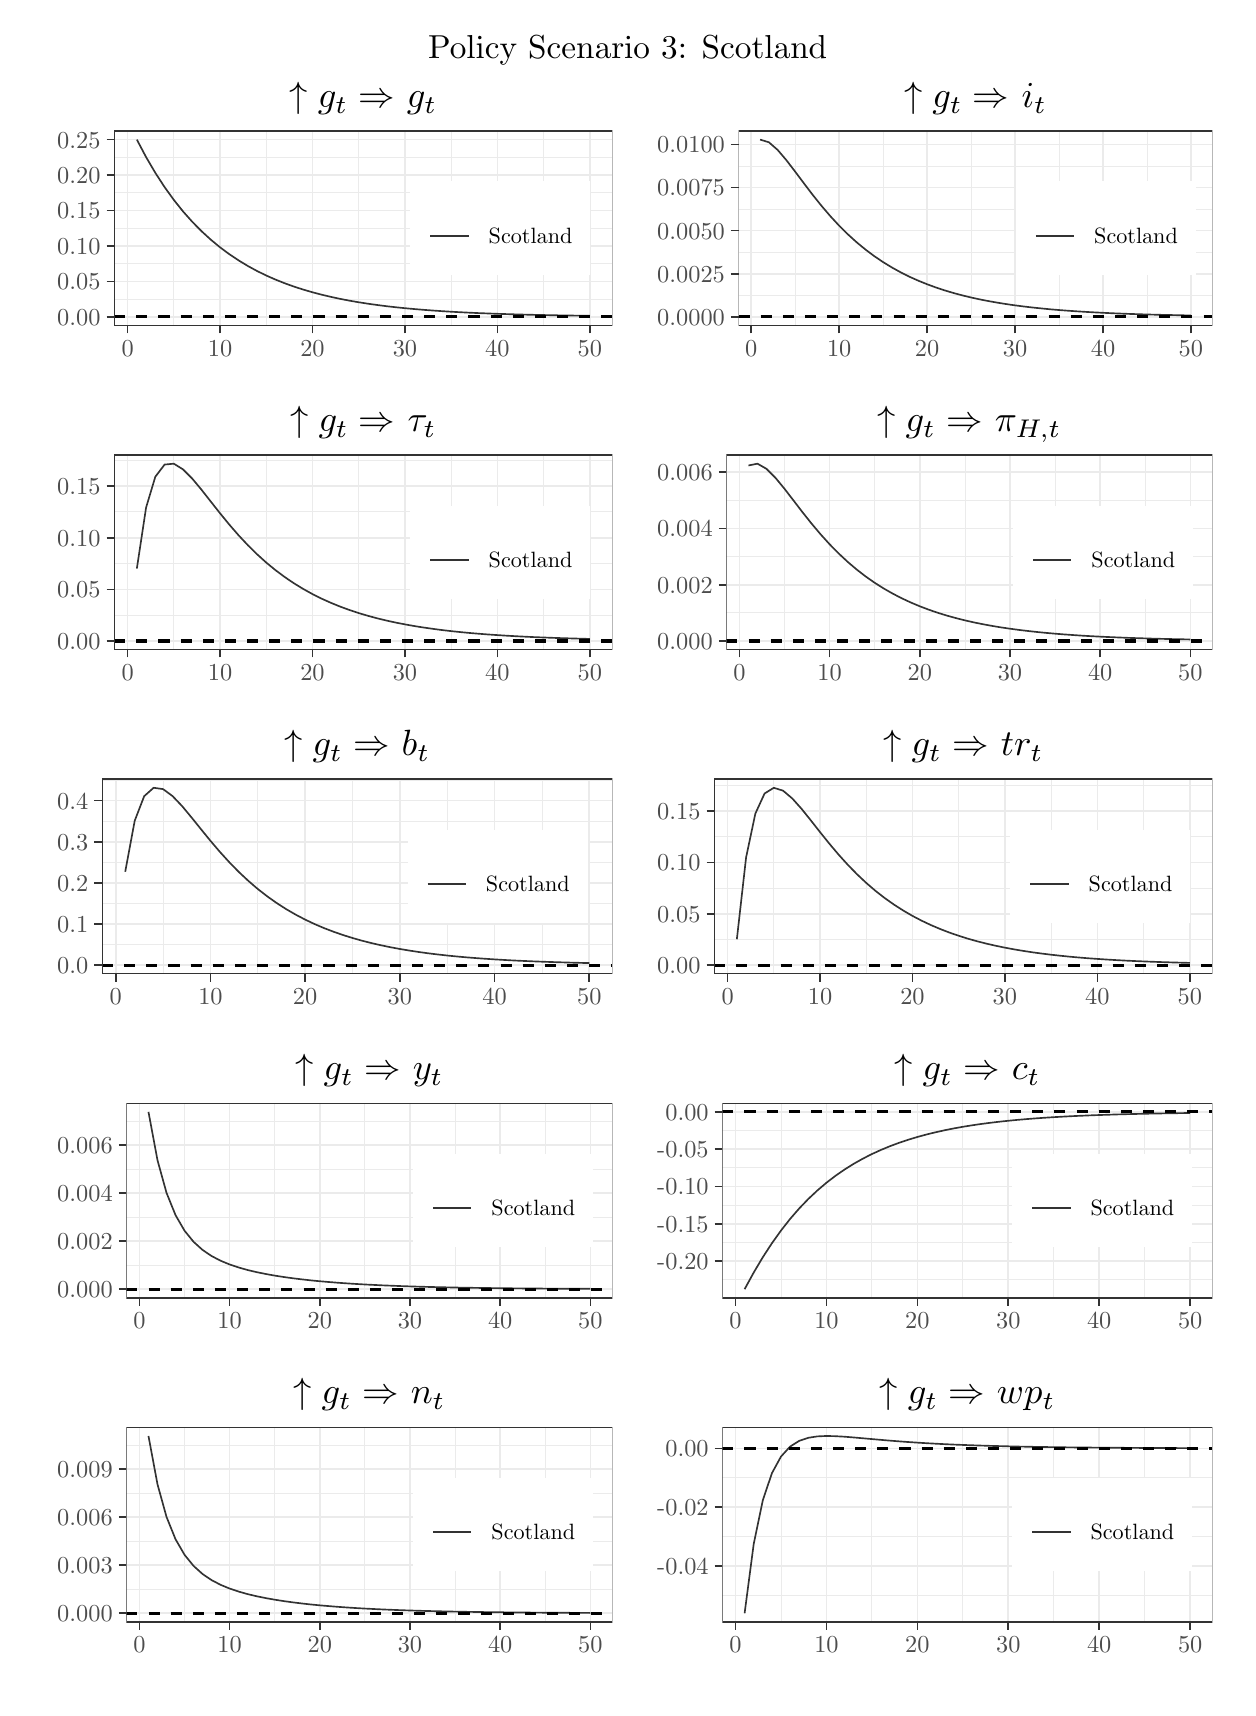
\begin{tikzpicture}[x=1pt,y=1pt]
\definecolor{fillColor}{RGB}{255,255,255}
\path[use as bounding box,fill=fillColor,fill opacity=0.00] (0,0) rectangle (433.62,599.84);
\begin{scope}
\path[clip] (  0.00,468.44) rectangle (216.81,585.55);
\definecolor{drawColor}{RGB}{255,255,255}
\definecolor{fillColor}{RGB}{255,255,255}

\path[draw=drawColor,line width= 0.6pt,line join=round,line cap=round,fill=fillColor] (  0.00,468.44) rectangle (216.81,585.55);
\end{scope}
\begin{scope}
\path[clip] ( 31.27,492.12) rectangle (211.31,562.59);
\definecolor{fillColor}{RGB}{255,255,255}

\path[fill=fillColor] ( 31.27,492.12) rectangle (211.31,562.59);
\definecolor{drawColor}{gray}{0.92}

\path[draw=drawColor,line width= 0.3pt,line join=round] ( 31.27,501.73) --
	(211.31,501.73);

\path[draw=drawColor,line width= 0.3pt,line join=round] ( 31.27,514.54) --
	(211.31,514.54);

\path[draw=drawColor,line width= 0.3pt,line join=round] ( 31.27,527.36) --
	(211.31,527.36);

\path[draw=drawColor,line width= 0.3pt,line join=round] ( 31.27,540.17) --
	(211.31,540.17);

\path[draw=drawColor,line width= 0.3pt,line join=round] ( 31.27,552.98) --
	(211.31,552.98);

\path[draw=drawColor,line width= 0.3pt,line join=round] ( 52.81,492.12) --
	( 52.81,562.59);

\path[draw=drawColor,line width= 0.3pt,line join=round] ( 86.22,492.12) --
	( 86.22,562.59);

\path[draw=drawColor,line width= 0.3pt,line join=round] (119.62,492.12) --
	(119.62,562.59);

\path[draw=drawColor,line width= 0.3pt,line join=round] (153.02,492.12) --
	(153.02,562.59);

\path[draw=drawColor,line width= 0.3pt,line join=round] (186.43,492.12) --
	(186.43,562.59);

\path[draw=drawColor,line width= 0.6pt,line join=round] ( 31.27,495.32) --
	(211.31,495.32);

\path[draw=drawColor,line width= 0.6pt,line join=round] ( 31.27,508.14) --
	(211.31,508.14);

\path[draw=drawColor,line width= 0.6pt,line join=round] ( 31.27,520.95) --
	(211.31,520.95);

\path[draw=drawColor,line width= 0.6pt,line join=round] ( 31.27,533.76) --
	(211.31,533.76);

\path[draw=drawColor,line width= 0.6pt,line join=round] ( 31.27,546.58) --
	(211.31,546.58);

\path[draw=drawColor,line width= 0.6pt,line join=round] ( 31.27,559.39) --
	(211.31,559.39);

\path[draw=drawColor,line width= 0.6pt,line join=round] ( 36.11,492.12) --
	( 36.11,562.59);

\path[draw=drawColor,line width= 0.6pt,line join=round] ( 69.52,492.12) --
	( 69.52,562.59);

\path[draw=drawColor,line width= 0.6pt,line join=round] (102.92,492.12) --
	(102.92,562.59);

\path[draw=drawColor,line width= 0.6pt,line join=round] (136.32,492.12) --
	(136.32,562.59);

\path[draw=drawColor,line width= 0.6pt,line join=round] (169.72,492.12) --
	(169.72,562.59);

\path[draw=drawColor,line width= 0.6pt,line join=round] (203.13,492.12) --
	(203.13,562.59);
\definecolor{drawColor}{gray}{0.20}

\path[draw=drawColor,line width= 0.6pt,line join=round] ( 39.45,559.39) --
	( 42.79,553.06) --
	( 46.13,547.37) --
	( 49.47,542.23) --
	( 52.81,537.60) --
	( 56.15,533.42) --
	( 59.50,529.66) --
	( 62.84,526.27) --
	( 66.18,523.22) --
	( 69.52,520.46) --
	( 72.86,517.98) --
	( 76.20,515.75) --
	( 79.54,513.73) --
	( 82.88,511.91) --
	( 86.22,510.27) --
	( 89.56,508.80) --
	( 92.90,507.47) --
	( 96.24,506.27) --
	( 99.58,505.19) --
	(102.92,504.22) --
	(106.26,503.34) --
	(109.60,502.55) --
	(112.94,501.83) --
	(116.28,501.19) --
	(119.62,500.61) --
	(122.96,500.09) --
	(126.30,499.62) --
	(129.64,499.19) --
	(132.98,498.81) --
	(136.32,498.47) --
	(139.66,498.16) --
	(143.00,497.88) --
	(146.34,497.63) --
	(149.68,497.40) --
	(153.02,497.19) --
	(156.36,497.01) --
	(159.70,496.84) --
	(163.04,496.69) --
	(166.38,496.56) --
	(169.72,496.44) --
	(173.06,496.33) --
	(176.40,496.23) --
	(179.74,496.14) --
	(183.08,496.06) --
	(186.43,495.99) --
	(189.77,495.92) --
	(193.11,495.86) --
	(196.45,495.81) --
	(199.79,495.76) --
	(203.13,495.72);
\definecolor{drawColor}{RGB}{0,0,0}

\path[draw=drawColor,line width= 1.1pt,dash pattern=on 4pt off 4pt ,line join=round] ( 31.27,495.32) -- (211.31,495.32);
\definecolor{drawColor}{gray}{0.20}

\path[draw=drawColor,line width= 0.6pt,line join=round,line cap=round] ( 31.27,492.12) rectangle (211.31,562.59);
\end{scope}
\begin{scope}
\path[clip] (  0.00,  0.00) rectangle (433.62,599.84);
\definecolor{drawColor}{gray}{0.30}

\node[text=drawColor,anchor=base east,inner sep=0pt, outer sep=0pt, scale=  0.88] at ( 26.32,492.29) {0.00};

\node[text=drawColor,anchor=base east,inner sep=0pt, outer sep=0pt, scale=  0.88] at ( 26.32,505.11) {0.05};

\node[text=drawColor,anchor=base east,inner sep=0pt, outer sep=0pt, scale=  0.88] at ( 26.32,517.92) {0.10};

\node[text=drawColor,anchor=base east,inner sep=0pt, outer sep=0pt, scale=  0.88] at ( 26.32,530.73) {0.15};

\node[text=drawColor,anchor=base east,inner sep=0pt, outer sep=0pt, scale=  0.88] at ( 26.32,543.55) {0.20};

\node[text=drawColor,anchor=base east,inner sep=0pt, outer sep=0pt, scale=  0.88] at ( 26.32,556.36) {0.25};
\end{scope}
\begin{scope}
\path[clip] (  0.00,  0.00) rectangle (433.62,599.84);
\definecolor{drawColor}{gray}{0.20}

\path[draw=drawColor,line width= 0.6pt,line join=round] ( 28.52,495.32) --
	( 31.27,495.32);

\path[draw=drawColor,line width= 0.6pt,line join=round] ( 28.52,508.14) --
	( 31.27,508.14);

\path[draw=drawColor,line width= 0.6pt,line join=round] ( 28.52,520.95) --
	( 31.27,520.95);

\path[draw=drawColor,line width= 0.6pt,line join=round] ( 28.52,533.76) --
	( 31.27,533.76);

\path[draw=drawColor,line width= 0.6pt,line join=round] ( 28.52,546.58) --
	( 31.27,546.58);

\path[draw=drawColor,line width= 0.6pt,line join=round] ( 28.52,559.39) --
	( 31.27,559.39);
\end{scope}
\begin{scope}
\path[clip] (  0.00,  0.00) rectangle (433.62,599.84);
\definecolor{drawColor}{gray}{0.20}

\path[draw=drawColor,line width= 0.6pt,line join=round] ( 36.11,489.37) --
	( 36.11,492.12);

\path[draw=drawColor,line width= 0.6pt,line join=round] ( 69.52,489.37) --
	( 69.52,492.12);

\path[draw=drawColor,line width= 0.6pt,line join=round] (102.92,489.37) --
	(102.92,492.12);

\path[draw=drawColor,line width= 0.6pt,line join=round] (136.32,489.37) --
	(136.32,492.12);

\path[draw=drawColor,line width= 0.6pt,line join=round] (169.72,489.37) --
	(169.72,492.12);

\path[draw=drawColor,line width= 0.6pt,line join=round] (203.13,489.37) --
	(203.13,492.12);
\end{scope}
\begin{scope}
\path[clip] (  0.00,  0.00) rectangle (433.62,599.84);
\definecolor{drawColor}{gray}{0.30}

\node[text=drawColor,anchor=base,inner sep=0pt, outer sep=0pt, scale=  0.88] at ( 36.11,481.11) {0};

\node[text=drawColor,anchor=base,inner sep=0pt, outer sep=0pt, scale=  0.88] at ( 69.52,481.11) {10};

\node[text=drawColor,anchor=base,inner sep=0pt, outer sep=0pt, scale=  0.88] at (102.92,481.11) {20};

\node[text=drawColor,anchor=base,inner sep=0pt, outer sep=0pt, scale=  0.88] at (136.32,481.11) {30};

\node[text=drawColor,anchor=base,inner sep=0pt, outer sep=0pt, scale=  0.88] at (169.72,481.11) {40};

\node[text=drawColor,anchor=base,inner sep=0pt, outer sep=0pt, scale=  0.88] at (203.13,481.11) {50};
\end{scope}
\begin{scope}
\path[clip] (  0.00,  0.00) rectangle (433.62,599.84);
\definecolor{fillColor}{RGB}{255,255,255}

\path[fill=fillColor] (138.26,510.43) rectangle (203.35,544.28);
\end{scope}
\begin{scope}
\path[clip] (  0.00,  0.00) rectangle (433.62,599.84);
\definecolor{fillColor}{RGB}{255,255,255}

\path[fill=fillColor] (143.76,515.93) rectangle (161.10,533.28);
\end{scope}
\begin{scope}
\path[clip] (  0.00,  0.00) rectangle (433.62,599.84);
\definecolor{drawColor}{gray}{0.20}

\path[draw=drawColor,line width= 0.6pt,line join=round] (145.49,524.61) -- (159.37,524.61);
\end{scope}
\begin{scope}
\path[clip] (  0.00,  0.00) rectangle (433.62,599.84);
\definecolor{drawColor}{RGB}{0,0,0}

\node[text=drawColor,anchor=base west,inner sep=0pt, outer sep=0pt, scale=  0.80] at (166.60,521.85) {Scotland};
\end{scope}
\begin{scope}
\path[clip] (  0.00,  0.00) rectangle (433.62,599.84);
\definecolor{drawColor}{RGB}{0,0,0}

\node[text=drawColor,anchor=base,inner sep=0pt, outer sep=0pt, scale=  1.32] at (121.29,570.96) {$\uparrow  g_t \Rightarrow $ ${g_t}$};
\end{scope}
\begin{scope}
\path[clip] (216.81,468.44) rectangle (433.62,585.55);
\definecolor{drawColor}{RGB}{255,255,255}
\definecolor{fillColor}{RGB}{255,255,255}

\path[draw=drawColor,line width= 0.6pt,line join=round,line cap=round,fill=fillColor] (216.81,468.44) rectangle (433.62,585.55);
\end{scope}
\begin{scope}
\path[clip] (256.88,492.12) rectangle (428.12,562.59);
\definecolor{fillColor}{RGB}{255,255,255}

\path[fill=fillColor] (256.88,492.12) rectangle (428.12,562.59);
\definecolor{drawColor}{gray}{0.92}

\path[draw=drawColor,line width= 0.3pt,line join=round] (256.88,503.12) --
	(428.12,503.12);

\path[draw=drawColor,line width= 0.3pt,line join=round] (256.88,518.70) --
	(428.12,518.70);

\path[draw=drawColor,line width= 0.3pt,line join=round] (256.88,534.29) --
	(428.12,534.29);

\path[draw=drawColor,line width= 0.3pt,line join=round] (256.88,549.87) --
	(428.12,549.87);

\path[draw=drawColor,line width= 0.3pt,line join=round] (277.37,492.12) --
	(277.37,562.59);

\path[draw=drawColor,line width= 0.3pt,line join=round] (309.14,492.12) --
	(309.14,562.59);

\path[draw=drawColor,line width= 0.3pt,line join=round] (340.91,492.12) --
	(340.91,562.59);

\path[draw=drawColor,line width= 0.3pt,line join=round] (372.68,492.12) --
	(372.68,562.59);

\path[draw=drawColor,line width= 0.3pt,line join=round] (404.45,492.12) --
	(404.45,562.59);

\path[draw=drawColor,line width= 0.6pt,line join=round] (256.88,495.32) --
	(428.12,495.32);

\path[draw=drawColor,line width= 0.6pt,line join=round] (256.88,510.91) --
	(428.12,510.91);

\path[draw=drawColor,line width= 0.6pt,line join=round] (256.88,526.50) --
	(428.12,526.50);

\path[draw=drawColor,line width= 0.6pt,line join=round] (256.88,542.08) --
	(428.12,542.08);

\path[draw=drawColor,line width= 0.6pt,line join=round] (256.88,557.67) --
	(428.12,557.67);

\path[draw=drawColor,line width= 0.6pt,line join=round] (261.48,492.12) --
	(261.48,562.59);

\path[draw=drawColor,line width= 0.6pt,line join=round] (293.25,492.12) --
	(293.25,562.59);

\path[draw=drawColor,line width= 0.6pt,line join=round] (325.03,492.12) --
	(325.03,562.59);

\path[draw=drawColor,line width= 0.6pt,line join=round] (356.80,492.12) --
	(356.80,562.59);

\path[draw=drawColor,line width= 0.6pt,line join=round] (388.57,492.12) --
	(388.57,562.59);

\path[draw=drawColor,line width= 0.6pt,line join=round] (420.34,492.12) --
	(420.34,562.59);
\definecolor{drawColor}{gray}{0.20}

\path[draw=drawColor,line width= 0.6pt,line join=round] (264.66,559.39) --
	(267.84,558.42) --
	(271.02,555.64) --
	(274.19,551.91) --
	(277.37,547.76) --
	(280.55,543.51) --
	(283.72,539.35) --
	(286.90,535.39) --
	(290.08,531.68) --
	(293.25,528.25) --
	(296.43,525.11) --
	(299.61,522.23) --
	(302.79,519.62) --
	(305.96,517.25) --
	(309.14,515.10) --
	(312.32,513.16) --
	(315.49,511.41) --
	(318.67,509.82) --
	(321.85,508.40) --
	(325.03,507.11) --
	(328.20,505.95) --
	(331.38,504.90) --
	(334.56,503.95) --
	(337.73,503.10) --
	(340.91,502.33) --
	(344.09,501.64) --
	(347.26,501.02) --
	(350.44,500.46) --
	(353.62,499.95) --
	(356.80,499.49) --
	(359.97,499.08) --
	(363.15,498.71) --
	(366.33,498.38) --
	(369.50,498.07) --
	(372.68,497.80) --
	(375.86,497.56) --
	(379.03,497.34) --
	(382.21,497.14) --
	(385.39,496.96) --
	(388.57,496.80) --
	(391.74,496.65) --
	(394.92,496.52) --
	(398.10,496.40) --
	(401.27,496.30) --
	(404.45,496.20) --
	(407.63,496.11) --
	(410.81,496.04) --
	(413.98,495.97) --
	(417.16,495.90) --
	(420.34,495.85);
\definecolor{drawColor}{RGB}{0,0,0}

\path[draw=drawColor,line width= 1.1pt,dash pattern=on 4pt off 4pt ,line join=round] (256.88,495.32) -- (428.12,495.32);
\definecolor{drawColor}{gray}{0.20}

\path[draw=drawColor,line width= 0.6pt,line join=round,line cap=round] (256.88,492.12) rectangle (428.12,562.59);
\end{scope}
\begin{scope}
\path[clip] (  0.00,  0.00) rectangle (433.62,599.84);
\definecolor{drawColor}{gray}{0.30}

\node[text=drawColor,anchor=base east,inner sep=0pt, outer sep=0pt, scale=  0.88] at (251.93,492.29) {0.0000};

\node[text=drawColor,anchor=base east,inner sep=0pt, outer sep=0pt, scale=  0.88] at (251.93,507.88) {0.0025};

\node[text=drawColor,anchor=base east,inner sep=0pt, outer sep=0pt, scale=  0.88] at (251.93,523.47) {0.0050};

\node[text=drawColor,anchor=base east,inner sep=0pt, outer sep=0pt, scale=  0.88] at (251.93,539.05) {0.0075};

\node[text=drawColor,anchor=base east,inner sep=0pt, outer sep=0pt, scale=  0.88] at (251.93,554.64) {0.0100};
\end{scope}
\begin{scope}
\path[clip] (  0.00,  0.00) rectangle (433.62,599.84);
\definecolor{drawColor}{gray}{0.20}

\path[draw=drawColor,line width= 0.6pt,line join=round] (254.13,495.32) --
	(256.88,495.32);

\path[draw=drawColor,line width= 0.6pt,line join=round] (254.13,510.91) --
	(256.88,510.91);

\path[draw=drawColor,line width= 0.6pt,line join=round] (254.13,526.50) --
	(256.88,526.50);

\path[draw=drawColor,line width= 0.6pt,line join=round] (254.13,542.08) --
	(256.88,542.08);

\path[draw=drawColor,line width= 0.6pt,line join=round] (254.13,557.67) --
	(256.88,557.67);
\end{scope}
\begin{scope}
\path[clip] (  0.00,  0.00) rectangle (433.62,599.84);
\definecolor{drawColor}{gray}{0.20}

\path[draw=drawColor,line width= 0.6pt,line join=round] (261.48,489.37) --
	(261.48,492.12);

\path[draw=drawColor,line width= 0.6pt,line join=round] (293.25,489.37) --
	(293.25,492.12);

\path[draw=drawColor,line width= 0.6pt,line join=round] (325.03,489.37) --
	(325.03,492.12);

\path[draw=drawColor,line width= 0.6pt,line join=round] (356.80,489.37) --
	(356.80,492.12);

\path[draw=drawColor,line width= 0.6pt,line join=round] (388.57,489.37) --
	(388.57,492.12);

\path[draw=drawColor,line width= 0.6pt,line join=round] (420.34,489.37) --
	(420.34,492.12);
\end{scope}
\begin{scope}
\path[clip] (  0.00,  0.00) rectangle (433.62,599.84);
\definecolor{drawColor}{gray}{0.30}

\node[text=drawColor,anchor=base,inner sep=0pt, outer sep=0pt, scale=  0.88] at (261.48,481.11) {0};

\node[text=drawColor,anchor=base,inner sep=0pt, outer sep=0pt, scale=  0.88] at (293.25,481.11) {10};

\node[text=drawColor,anchor=base,inner sep=0pt, outer sep=0pt, scale=  0.88] at (325.03,481.11) {20};

\node[text=drawColor,anchor=base,inner sep=0pt, outer sep=0pt, scale=  0.88] at (356.80,481.11) {30};

\node[text=drawColor,anchor=base,inner sep=0pt, outer sep=0pt, scale=  0.88] at (388.57,481.11) {40};

\node[text=drawColor,anchor=base,inner sep=0pt, outer sep=0pt, scale=  0.88] at (420.34,481.11) {50};
\end{scope}
\begin{scope}
\path[clip] (  0.00,  0.00) rectangle (433.62,599.84);
\definecolor{fillColor}{RGB}{255,255,255}

\path[fill=fillColor] (357.05,510.43) rectangle (422.14,544.28);
\end{scope}
\begin{scope}
\path[clip] (  0.00,  0.00) rectangle (433.62,599.84);
\definecolor{fillColor}{RGB}{255,255,255}

\path[fill=fillColor] (362.55,515.93) rectangle (379.89,533.28);
\end{scope}
\begin{scope}
\path[clip] (  0.00,  0.00) rectangle (433.62,599.84);
\definecolor{drawColor}{gray}{0.20}

\path[draw=drawColor,line width= 0.6pt,line join=round] (364.28,524.61) -- (378.16,524.61);
\end{scope}
\begin{scope}
\path[clip] (  0.00,  0.00) rectangle (433.62,599.84);
\definecolor{drawColor}{RGB}{0,0,0}

\node[text=drawColor,anchor=base west,inner sep=0pt, outer sep=0pt, scale=  0.80] at (385.39,521.85) {Scotland};
\end{scope}
\begin{scope}
\path[clip] (  0.00,  0.00) rectangle (433.62,599.84);
\definecolor{drawColor}{RGB}{0,0,0}

\node[text=drawColor,anchor=base,inner sep=0pt, outer sep=0pt, scale=  1.32] at (342.50,570.96) {$\uparrow  g_t \Rightarrow $ ${i_t}$};
\end{scope}
\begin{scope}
\path[clip] (  0.00,351.33) rectangle (216.81,468.44);
\definecolor{drawColor}{RGB}{255,255,255}
\definecolor{fillColor}{RGB}{255,255,255}

\path[draw=drawColor,line width= 0.6pt,line join=round,line cap=round,fill=fillColor] (  0.00,351.33) rectangle (216.81,468.44);
\end{scope}
\begin{scope}
\path[clip] ( 31.27,375.01) rectangle (211.31,445.48);
\definecolor{fillColor}{RGB}{255,255,255}

\path[fill=fillColor] ( 31.27,375.01) rectangle (211.31,445.48);
\definecolor{drawColor}{gray}{0.92}

\path[draw=drawColor,line width= 0.3pt,line join=round] ( 31.27,387.54) --
	(211.31,387.54);

\path[draw=drawColor,line width= 0.3pt,line join=round] ( 31.27,406.20) --
	(211.31,406.20);

\path[draw=drawColor,line width= 0.3pt,line join=round] ( 31.27,424.86) --
	(211.31,424.86);

\path[draw=drawColor,line width= 0.3pt,line join=round] ( 31.27,443.52) --
	(211.31,443.52);

\path[draw=drawColor,line width= 0.3pt,line join=round] ( 52.81,375.01) --
	( 52.81,445.48);

\path[draw=drawColor,line width= 0.3pt,line join=round] ( 86.22,375.01) --
	( 86.22,445.48);

\path[draw=drawColor,line width= 0.3pt,line join=round] (119.62,375.01) --
	(119.62,445.48);

\path[draw=drawColor,line width= 0.3pt,line join=round] (153.02,375.01) --
	(153.02,445.48);

\path[draw=drawColor,line width= 0.3pt,line join=round] (186.43,375.01) --
	(186.43,445.48);

\path[draw=drawColor,line width= 0.6pt,line join=round] ( 31.27,378.21) --
	(211.31,378.21);

\path[draw=drawColor,line width= 0.6pt,line join=round] ( 31.27,396.87) --
	(211.31,396.87);

\path[draw=drawColor,line width= 0.6pt,line join=round] ( 31.27,415.53) --
	(211.31,415.53);

\path[draw=drawColor,line width= 0.6pt,line join=round] ( 31.27,434.19) --
	(211.31,434.19);

\path[draw=drawColor,line width= 0.6pt,line join=round] ( 36.11,375.01) --
	( 36.11,445.48);

\path[draw=drawColor,line width= 0.6pt,line join=round] ( 69.52,375.01) --
	( 69.52,445.48);

\path[draw=drawColor,line width= 0.6pt,line join=round] (102.92,375.01) --
	(102.92,445.48);

\path[draw=drawColor,line width= 0.6pt,line join=round] (136.32,375.01) --
	(136.32,445.48);

\path[draw=drawColor,line width= 0.6pt,line join=round] (169.72,375.01) --
	(169.72,445.48);

\path[draw=drawColor,line width= 0.6pt,line join=round] (203.13,375.01) --
	(203.13,445.48);
\definecolor{drawColor}{gray}{0.20}

\path[draw=drawColor,line width= 0.6pt,line join=round] ( 39.45,404.38) --
	( 42.79,426.44) --
	( 46.13,437.57) --
	( 49.47,441.96) --
	( 52.81,442.28) --
	( 56.15,440.21) --
	( 59.50,436.84) --
	( 62.84,432.83) --
	( 66.18,428.58) --
	( 69.52,424.35) --
	( 72.86,420.27) --
	( 76.20,416.42) --
	( 79.54,412.85) --
	( 82.88,409.56) --
	( 86.22,406.54) --
	( 89.56,403.80) --
	( 92.90,401.31) --
	( 96.24,399.05) --
	( 99.58,397.01) --
	(102.92,395.16) --
	(106.26,393.49) --
	(109.60,391.99) --
	(112.94,390.63) --
	(116.28,389.41) --
	(119.62,388.30) --
	(122.96,387.31) --
	(126.30,386.41) --
	(129.64,385.60) --
	(132.98,384.87) --
	(136.32,384.22) --
	(139.66,383.62) --
	(143.00,383.09) --
	(146.34,382.61) --
	(149.68,382.17) --
	(153.02,381.78) --
	(156.36,381.43) --
	(159.70,381.11) --
	(163.04,380.83) --
	(166.38,380.57) --
	(169.72,380.34) --
	(173.06,380.13) --
	(176.40,379.94) --
	(179.74,379.77) --
	(183.08,379.61) --
	(186.43,379.48) --
	(189.77,379.35) --
	(193.11,379.24) --
	(196.45,379.14) --
	(199.79,379.05) --
	(203.13,378.96);
\definecolor{drawColor}{RGB}{0,0,0}

\path[draw=drawColor,line width= 1.1pt,dash pattern=on 4pt off 4pt ,line join=round] ( 31.27,378.21) -- (211.31,378.21);
\definecolor{drawColor}{gray}{0.20}

\path[draw=drawColor,line width= 0.6pt,line join=round,line cap=round] ( 31.27,375.01) rectangle (211.31,445.48);
\end{scope}
\begin{scope}
\path[clip] (  0.00,  0.00) rectangle (433.62,599.84);
\definecolor{drawColor}{gray}{0.30}

\node[text=drawColor,anchor=base east,inner sep=0pt, outer sep=0pt, scale=  0.88] at ( 26.32,375.18) {0.00};

\node[text=drawColor,anchor=base east,inner sep=0pt, outer sep=0pt, scale=  0.88] at ( 26.32,393.84) {0.05};

\node[text=drawColor,anchor=base east,inner sep=0pt, outer sep=0pt, scale=  0.88] at ( 26.32,412.50) {0.10};

\node[text=drawColor,anchor=base east,inner sep=0pt, outer sep=0pt, scale=  0.88] at ( 26.32,431.16) {0.15};
\end{scope}
\begin{scope}
\path[clip] (  0.00,  0.00) rectangle (433.62,599.84);
\definecolor{drawColor}{gray}{0.20}

\path[draw=drawColor,line width= 0.6pt,line join=round] ( 28.52,378.21) --
	( 31.27,378.21);

\path[draw=drawColor,line width= 0.6pt,line join=round] ( 28.52,396.87) --
	( 31.27,396.87);

\path[draw=drawColor,line width= 0.6pt,line join=round] ( 28.52,415.53) --
	( 31.27,415.53);

\path[draw=drawColor,line width= 0.6pt,line join=round] ( 28.52,434.19) --
	( 31.27,434.19);
\end{scope}
\begin{scope}
\path[clip] (  0.00,  0.00) rectangle (433.62,599.84);
\definecolor{drawColor}{gray}{0.20}

\path[draw=drawColor,line width= 0.6pt,line join=round] ( 36.11,372.26) --
	( 36.11,375.01);

\path[draw=drawColor,line width= 0.6pt,line join=round] ( 69.52,372.26) --
	( 69.52,375.01);

\path[draw=drawColor,line width= 0.6pt,line join=round] (102.92,372.26) --
	(102.92,375.01);

\path[draw=drawColor,line width= 0.6pt,line join=round] (136.32,372.26) --
	(136.32,375.01);

\path[draw=drawColor,line width= 0.6pt,line join=round] (169.72,372.26) --
	(169.72,375.01);

\path[draw=drawColor,line width= 0.6pt,line join=round] (203.13,372.26) --
	(203.13,375.01);
\end{scope}
\begin{scope}
\path[clip] (  0.00,  0.00) rectangle (433.62,599.84);
\definecolor{drawColor}{gray}{0.30}

\node[text=drawColor,anchor=base,inner sep=0pt, outer sep=0pt, scale=  0.88] at ( 36.11,364.00) {0};

\node[text=drawColor,anchor=base,inner sep=0pt, outer sep=0pt, scale=  0.88] at ( 69.52,364.00) {10};

\node[text=drawColor,anchor=base,inner sep=0pt, outer sep=0pt, scale=  0.88] at (102.92,364.00) {20};

\node[text=drawColor,anchor=base,inner sep=0pt, outer sep=0pt, scale=  0.88] at (136.32,364.00) {30};

\node[text=drawColor,anchor=base,inner sep=0pt, outer sep=0pt, scale=  0.88] at (169.72,364.00) {40};

\node[text=drawColor,anchor=base,inner sep=0pt, outer sep=0pt, scale=  0.88] at (203.13,364.00) {50};
\end{scope}
\begin{scope}
\path[clip] (  0.00,  0.00) rectangle (433.62,599.84);
\definecolor{fillColor}{RGB}{255,255,255}

\path[fill=fillColor] (138.26,393.32) rectangle (203.35,427.17);
\end{scope}
\begin{scope}
\path[clip] (  0.00,  0.00) rectangle (433.62,599.84);
\definecolor{fillColor}{RGB}{255,255,255}

\path[fill=fillColor] (143.76,398.82) rectangle (161.10,416.17);
\end{scope}
\begin{scope}
\path[clip] (  0.00,  0.00) rectangle (433.62,599.84);
\definecolor{drawColor}{gray}{0.20}

\path[draw=drawColor,line width= 0.6pt,line join=round] (145.49,407.50) -- (159.37,407.50);
\end{scope}
\begin{scope}
\path[clip] (  0.00,  0.00) rectangle (433.62,599.84);
\definecolor{drawColor}{RGB}{0,0,0}

\node[text=drawColor,anchor=base west,inner sep=0pt, outer sep=0pt, scale=  0.80] at (166.60,404.74) {Scotland};
\end{scope}
\begin{scope}
\path[clip] (  0.00,  0.00) rectangle (433.62,599.84);
\definecolor{drawColor}{RGB}{0,0,0}

\node[text=drawColor,anchor=base,inner sep=0pt, outer sep=0pt, scale=  1.32] at (121.29,453.85) {$\uparrow  g_t \Rightarrow $ ${\tau_t}$};
\end{scope}
\begin{scope}
\path[clip] (216.81,351.33) rectangle (433.62,468.44);
\definecolor{drawColor}{RGB}{255,255,255}
\definecolor{fillColor}{RGB}{255,255,255}

\path[draw=drawColor,line width= 0.6pt,line join=round,line cap=round,fill=fillColor] (216.81,351.33) rectangle (433.62,468.44);
\end{scope}
\begin{scope}
\path[clip] (252.48,375.01) rectangle (428.12,445.48);
\definecolor{fillColor}{RGB}{255,255,255}

\path[fill=fillColor] (252.48,375.01) rectangle (428.12,445.48);
\definecolor{drawColor}{gray}{0.92}

\path[draw=drawColor,line width= 0.3pt,line join=round] (252.48,388.38) --
	(428.12,388.38);

\path[draw=drawColor,line width= 0.3pt,line join=round] (252.48,408.72) --
	(428.12,408.72);

\path[draw=drawColor,line width= 0.3pt,line join=round] (252.48,429.06) --
	(428.12,429.06);

\path[draw=drawColor,line width= 0.3pt,line join=round] (273.50,375.01) --
	(273.50,445.48);

\path[draw=drawColor,line width= 0.3pt,line join=round] (306.08,375.01) --
	(306.08,445.48);

\path[draw=drawColor,line width= 0.3pt,line join=round] (338.67,375.01) --
	(338.67,445.48);

\path[draw=drawColor,line width= 0.3pt,line join=round] (371.26,375.01) --
	(371.26,445.48);

\path[draw=drawColor,line width= 0.3pt,line join=round] (403.84,375.01) --
	(403.84,445.48);

\path[draw=drawColor,line width= 0.6pt,line join=round] (252.48,378.21) --
	(428.12,378.21);

\path[draw=drawColor,line width= 0.6pt,line join=round] (252.48,398.55) --
	(428.12,398.55);

\path[draw=drawColor,line width= 0.6pt,line join=round] (252.48,418.89) --
	(428.12,418.89);

\path[draw=drawColor,line width= 0.6pt,line join=round] (252.48,439.23) --
	(428.12,439.23);

\path[draw=drawColor,line width= 0.6pt,line join=round] (257.20,375.01) --
	(257.20,445.48);

\path[draw=drawColor,line width= 0.6pt,line join=round] (289.79,375.01) --
	(289.79,445.48);

\path[draw=drawColor,line width= 0.6pt,line join=round] (322.38,375.01) --
	(322.38,445.48);

\path[draw=drawColor,line width= 0.6pt,line join=round] (354.96,375.01) --
	(354.96,445.48);

\path[draw=drawColor,line width= 0.6pt,line join=round] (387.55,375.01) --
	(387.55,445.48);

\path[draw=drawColor,line width= 0.6pt,line join=round] (420.14,375.01) --
	(420.14,445.48);
\definecolor{drawColor}{gray}{0.20}

\path[draw=drawColor,line width= 0.6pt,line join=round] (260.46,441.63) --
	(263.72,442.28) --
	(266.98,440.41) --
	(270.24,437.14) --
	(273.50,433.18) --
	(276.76,428.95) --
	(280.01,424.71) --
	(283.27,420.62) --
	(286.53,416.75) --
	(289.79,413.15) --
	(293.05,409.84) --
	(296.31,406.80) --
	(299.57,404.03) --
	(302.82,401.52) --
	(306.08,399.24) --
	(309.34,397.18) --
	(312.60,395.32) --
	(315.86,393.64) --
	(319.12,392.12) --
	(322.38,390.75) --
	(325.64,389.51) --
	(328.89,388.40) --
	(332.15,387.39) --
	(335.41,386.49) --
	(338.67,385.67) --
	(341.93,384.93) --
	(345.19,384.27) --
	(348.45,383.67) --
	(351.70,383.13) --
	(354.96,382.65) --
	(358.22,382.21) --
	(361.48,381.82) --
	(364.74,381.46) --
	(368.00,381.14) --
	(371.26,380.85) --
	(374.52,380.59) --
	(377.77,380.36) --
	(381.03,380.14) --
	(384.29,379.95) --
	(387.55,379.78) --
	(390.81,379.63) --
	(394.07,379.49) --
	(397.33,379.36) --
	(400.58,379.25) --
	(403.84,379.15) --
	(407.10,379.05) --
	(410.36,378.97) --
	(413.62,378.90) --
	(416.88,378.83) --
	(420.14,378.77);
\definecolor{drawColor}{RGB}{0,0,0}

\path[draw=drawColor,line width= 1.1pt,dash pattern=on 4pt off 4pt ,line join=round] (252.48,378.21) -- (428.12,378.21);
\definecolor{drawColor}{gray}{0.20}

\path[draw=drawColor,line width= 0.6pt,line join=round,line cap=round] (252.48,375.01) rectangle (428.12,445.48);
\end{scope}
\begin{scope}
\path[clip] (  0.00,  0.00) rectangle (433.62,599.84);
\definecolor{drawColor}{gray}{0.30}

\node[text=drawColor,anchor=base east,inner sep=0pt, outer sep=0pt, scale=  0.88] at (247.53,375.18) {0.000};

\node[text=drawColor,anchor=base east,inner sep=0pt, outer sep=0pt, scale=  0.88] at (247.53,395.52) {0.002};

\node[text=drawColor,anchor=base east,inner sep=0pt, outer sep=0pt, scale=  0.88] at (247.53,415.86) {0.004};

\node[text=drawColor,anchor=base east,inner sep=0pt, outer sep=0pt, scale=  0.88] at (247.53,436.20) {0.006};
\end{scope}
\begin{scope}
\path[clip] (  0.00,  0.00) rectangle (433.62,599.84);
\definecolor{drawColor}{gray}{0.20}

\path[draw=drawColor,line width= 0.6pt,line join=round] (249.73,378.21) --
	(252.48,378.21);

\path[draw=drawColor,line width= 0.6pt,line join=round] (249.73,398.55) --
	(252.48,398.55);

\path[draw=drawColor,line width= 0.6pt,line join=round] (249.73,418.89) --
	(252.48,418.89);

\path[draw=drawColor,line width= 0.6pt,line join=round] (249.73,439.23) --
	(252.48,439.23);
\end{scope}
\begin{scope}
\path[clip] (  0.00,  0.00) rectangle (433.62,599.84);
\definecolor{drawColor}{gray}{0.20}

\path[draw=drawColor,line width= 0.6pt,line join=round] (257.20,372.26) --
	(257.20,375.01);

\path[draw=drawColor,line width= 0.6pt,line join=round] (289.79,372.26) --
	(289.79,375.01);

\path[draw=drawColor,line width= 0.6pt,line join=round] (322.38,372.26) --
	(322.38,375.01);

\path[draw=drawColor,line width= 0.6pt,line join=round] (354.96,372.26) --
	(354.96,375.01);

\path[draw=drawColor,line width= 0.6pt,line join=round] (387.55,372.26) --
	(387.55,375.01);

\path[draw=drawColor,line width= 0.6pt,line join=round] (420.14,372.26) --
	(420.14,375.01);
\end{scope}
\begin{scope}
\path[clip] (  0.00,  0.00) rectangle (433.62,599.84);
\definecolor{drawColor}{gray}{0.30}

\node[text=drawColor,anchor=base,inner sep=0pt, outer sep=0pt, scale=  0.88] at (257.20,364.00) {0};

\node[text=drawColor,anchor=base,inner sep=0pt, outer sep=0pt, scale=  0.88] at (289.79,364.00) {10};

\node[text=drawColor,anchor=base,inner sep=0pt, outer sep=0pt, scale=  0.88] at (322.38,364.00) {20};

\node[text=drawColor,anchor=base,inner sep=0pt, outer sep=0pt, scale=  0.88] at (354.96,364.00) {30};

\node[text=drawColor,anchor=base,inner sep=0pt, outer sep=0pt, scale=  0.88] at (387.55,364.00) {40};

\node[text=drawColor,anchor=base,inner sep=0pt, outer sep=0pt, scale=  0.88] at (420.14,364.00) {50};
\end{scope}
\begin{scope}
\path[clip] (  0.00,  0.00) rectangle (433.62,599.84);
\definecolor{fillColor}{RGB}{255,255,255}

\path[fill=fillColor] (356.06,393.32) rectangle (421.15,427.17);
\end{scope}
\begin{scope}
\path[clip] (  0.00,  0.00) rectangle (433.62,599.84);
\definecolor{fillColor}{RGB}{255,255,255}

\path[fill=fillColor] (361.56,398.82) rectangle (378.90,416.17);
\end{scope}
\begin{scope}
\path[clip] (  0.00,  0.00) rectangle (433.62,599.84);
\definecolor{drawColor}{gray}{0.20}

\path[draw=drawColor,line width= 0.6pt,line join=round] (363.29,407.50) -- (377.17,407.50);
\end{scope}
\begin{scope}
\path[clip] (  0.00,  0.00) rectangle (433.62,599.84);
\definecolor{drawColor}{RGB}{0,0,0}

\node[text=drawColor,anchor=base west,inner sep=0pt, outer sep=0pt, scale=  0.80] at (384.40,404.74) {Scotland};
\end{scope}
\begin{scope}
\path[clip] (  0.00,  0.00) rectangle (433.62,599.84);
\definecolor{drawColor}{RGB}{0,0,0}

\node[text=drawColor,anchor=base,inner sep=0pt, outer sep=0pt, scale=  1.32] at (340.30,453.85) {$\uparrow  g_t \Rightarrow $ ${\pi_{H,t}}$};
\end{scope}
\begin{scope}
\path[clip] (  0.00,234.22) rectangle (216.81,351.33);
\definecolor{drawColor}{RGB}{255,255,255}
\definecolor{fillColor}{RGB}{255,255,255}

\path[draw=drawColor,line width= 0.6pt,line join=round,line cap=round,fill=fillColor] (  0.00,234.22) rectangle (216.81,351.33);
\end{scope}
\begin{scope}
\path[clip] ( 26.87,257.90) rectangle (211.31,328.37);
\definecolor{fillColor}{RGB}{255,255,255}

\path[fill=fillColor] ( 26.87,257.90) rectangle (211.31,328.37);
\definecolor{drawColor}{gray}{0.92}

\path[draw=drawColor,line width= 0.3pt,line join=round] ( 26.87,268.53) --
	(211.31,268.53);

\path[draw=drawColor,line width= 0.3pt,line join=round] ( 26.87,283.38) --
	(211.31,283.38);

\path[draw=drawColor,line width= 0.3pt,line join=round] ( 26.87,298.24) --
	(211.31,298.24);

\path[draw=drawColor,line width= 0.3pt,line join=round] ( 26.87,313.09) --
	(211.31,313.09);

\path[draw=drawColor,line width= 0.3pt,line join=round] ( 26.87,327.94) --
	(211.31,327.94);

\path[draw=drawColor,line width= 0.3pt,line join=round] ( 48.94,257.90) --
	( 48.94,328.37);

\path[draw=drawColor,line width= 0.3pt,line join=round] ( 83.16,257.90) --
	( 83.16,328.37);

\path[draw=drawColor,line width= 0.3pt,line join=round] (117.38,257.90) --
	(117.38,328.37);

\path[draw=drawColor,line width= 0.3pt,line join=round] (151.60,257.90) --
	(151.60,328.37);

\path[draw=drawColor,line width= 0.3pt,line join=round] (185.82,257.90) --
	(185.82,328.37);

\path[draw=drawColor,line width= 0.6pt,line join=round] ( 26.87,261.10) --
	(211.31,261.10);

\path[draw=drawColor,line width= 0.6pt,line join=round] ( 26.87,275.96) --
	(211.31,275.96);

\path[draw=drawColor,line width= 0.6pt,line join=round] ( 26.87,290.81) --
	(211.31,290.81);

\path[draw=drawColor,line width= 0.6pt,line join=round] ( 26.87,305.66) --
	(211.31,305.66);

\path[draw=drawColor,line width= 0.6pt,line join=round] ( 26.87,320.52) --
	(211.31,320.52);

\path[draw=drawColor,line width= 0.6pt,line join=round] ( 31.83,257.90) --
	( 31.83,328.37);

\path[draw=drawColor,line width= 0.6pt,line join=round] ( 66.05,257.90) --
	( 66.05,328.37);

\path[draw=drawColor,line width= 0.6pt,line join=round] (100.27,257.90) --
	(100.27,328.37);

\path[draw=drawColor,line width= 0.6pt,line join=round] (134.49,257.90) --
	(134.49,328.37);

\path[draw=drawColor,line width= 0.6pt,line join=round] (168.71,257.90) --
	(168.71,328.37);

\path[draw=drawColor,line width= 0.6pt,line join=round] (202.93,257.90) --
	(202.93,328.37);
\definecolor{drawColor}{gray}{0.20}

\path[draw=drawColor,line width= 0.6pt,line join=round] ( 35.25,294.84) --
	( 38.68,313.26) --
	( 42.10,322.14) --
	( 45.52,325.17) --
	( 48.94,324.68) --
	( 52.36,322.16) --
	( 55.79,318.56) --
	( 59.21,314.45) --
	( 62.63,310.20) --
	( 66.05,306.00) --
	( 69.47,301.99) --
	( 72.90,298.22) --
	( 76.32,294.73) --
	( 79.74,291.53) --
	( 83.16,288.59) --
	( 86.58,285.93) --
	( 90.00,283.51) --
	( 93.43,281.31) --
	( 96.85,279.33) --
	(100.27,277.54) --
	(103.69,275.92) --
	(107.11,274.46) --
	(110.54,273.15) --
	(113.96,271.96) --
	(117.38,270.89) --
	(120.80,269.92) --
	(124.22,269.05) --
	(127.65,268.27) --
	(131.07,267.56) --
	(134.49,266.92) --
	(137.91,266.35) --
	(141.33,265.83) --
	(144.75,265.36) --
	(148.18,264.94) --
	(151.60,264.56) --
	(155.02,264.22) --
	(158.44,263.91) --
	(161.86,263.64) --
	(165.29,263.39) --
	(168.71,263.16) --
	(172.13,262.96) --
	(175.55,262.77) --
	(178.97,262.61) --
	(182.40,262.46) --
	(185.82,262.33) --
	(189.24,262.21) --
	(192.66,262.10) --
	(196.08,262.00) --
	(199.50,261.91) --
	(202.93,261.83);
\definecolor{drawColor}{RGB}{0,0,0}

\path[draw=drawColor,line width= 1.1pt,dash pattern=on 4pt off 4pt ,line join=round] ( 26.87,261.10) -- (211.31,261.10);
\definecolor{drawColor}{gray}{0.20}

\path[draw=drawColor,line width= 0.6pt,line join=round,line cap=round] ( 26.87,257.90) rectangle (211.31,328.37);
\end{scope}
\begin{scope}
\path[clip] (  0.00,  0.00) rectangle (433.62,599.84);
\definecolor{drawColor}{gray}{0.30}

\node[text=drawColor,anchor=base east,inner sep=0pt, outer sep=0pt, scale=  0.88] at ( 21.92,258.07) {0.0};

\node[text=drawColor,anchor=base east,inner sep=0pt, outer sep=0pt, scale=  0.88] at ( 21.92,272.93) {0.1};

\node[text=drawColor,anchor=base east,inner sep=0pt, outer sep=0pt, scale=  0.88] at ( 21.92,287.78) {0.2};

\node[text=drawColor,anchor=base east,inner sep=0pt, outer sep=0pt, scale=  0.88] at ( 21.92,302.63) {0.3};

\node[text=drawColor,anchor=base east,inner sep=0pt, outer sep=0pt, scale=  0.88] at ( 21.92,317.49) {0.4};
\end{scope}
\begin{scope}
\path[clip] (  0.00,  0.00) rectangle (433.62,599.84);
\definecolor{drawColor}{gray}{0.20}

\path[draw=drawColor,line width= 0.6pt,line join=round] ( 24.12,261.10) --
	( 26.87,261.10);

\path[draw=drawColor,line width= 0.6pt,line join=round] ( 24.12,275.96) --
	( 26.87,275.96);

\path[draw=drawColor,line width= 0.6pt,line join=round] ( 24.12,290.81) --
	( 26.87,290.81);

\path[draw=drawColor,line width= 0.6pt,line join=round] ( 24.12,305.66) --
	( 26.87,305.66);

\path[draw=drawColor,line width= 0.6pt,line join=round] ( 24.12,320.52) --
	( 26.87,320.52);
\end{scope}
\begin{scope}
\path[clip] (  0.00,  0.00) rectangle (433.62,599.84);
\definecolor{drawColor}{gray}{0.20}

\path[draw=drawColor,line width= 0.6pt,line join=round] ( 31.83,255.15) --
	( 31.83,257.90);

\path[draw=drawColor,line width= 0.6pt,line join=round] ( 66.05,255.15) --
	( 66.05,257.90);

\path[draw=drawColor,line width= 0.6pt,line join=round] (100.27,255.15) --
	(100.27,257.90);

\path[draw=drawColor,line width= 0.6pt,line join=round] (134.49,255.15) --
	(134.49,257.90);

\path[draw=drawColor,line width= 0.6pt,line join=round] (168.71,255.15) --
	(168.71,257.90);

\path[draw=drawColor,line width= 0.6pt,line join=round] (202.93,255.15) --
	(202.93,257.90);
\end{scope}
\begin{scope}
\path[clip] (  0.00,  0.00) rectangle (433.62,599.84);
\definecolor{drawColor}{gray}{0.30}

\node[text=drawColor,anchor=base,inner sep=0pt, outer sep=0pt, scale=  0.88] at ( 31.83,246.89) {0};

\node[text=drawColor,anchor=base,inner sep=0pt, outer sep=0pt, scale=  0.88] at ( 66.05,246.89) {10};

\node[text=drawColor,anchor=base,inner sep=0pt, outer sep=0pt, scale=  0.88] at (100.27,246.89) {20};

\node[text=drawColor,anchor=base,inner sep=0pt, outer sep=0pt, scale=  0.88] at (134.49,246.89) {30};

\node[text=drawColor,anchor=base,inner sep=0pt, outer sep=0pt, scale=  0.88] at (168.71,246.89) {40};

\node[text=drawColor,anchor=base,inner sep=0pt, outer sep=0pt, scale=  0.88] at (202.93,246.89) {50};
\end{scope}
\begin{scope}
\path[clip] (  0.00,  0.00) rectangle (433.62,599.84);
\definecolor{fillColor}{RGB}{255,255,255}

\path[fill=fillColor] (137.27,276.21) rectangle (202.36,310.06);
\end{scope}
\begin{scope}
\path[clip] (  0.00,  0.00) rectangle (433.62,599.84);
\definecolor{fillColor}{RGB}{255,255,255}

\path[fill=fillColor] (142.77,281.71) rectangle (160.11,299.06);
\end{scope}
\begin{scope}
\path[clip] (  0.00,  0.00) rectangle (433.62,599.84);
\definecolor{drawColor}{gray}{0.20}

\path[draw=drawColor,line width= 0.6pt,line join=round] (144.50,290.38) -- (158.38,290.38);
\end{scope}
\begin{scope}
\path[clip] (  0.00,  0.00) rectangle (433.62,599.84);
\definecolor{drawColor}{RGB}{0,0,0}

\node[text=drawColor,anchor=base west,inner sep=0pt, outer sep=0pt, scale=  0.80] at (165.61,287.63) {Scotland};
\end{scope}
\begin{scope}
\path[clip] (  0.00,  0.00) rectangle (433.62,599.84);
\definecolor{drawColor}{RGB}{0,0,0}

\node[text=drawColor,anchor=base,inner sep=0pt, outer sep=0pt, scale=  1.32] at (119.09,336.74) {$\uparrow  g_t \Rightarrow $ ${b_t}$};
\end{scope}
\begin{scope}
\path[clip] (216.81,234.22) rectangle (433.62,351.33);
\definecolor{drawColor}{RGB}{255,255,255}
\definecolor{fillColor}{RGB}{255,255,255}

\path[draw=drawColor,line width= 0.6pt,line join=round,line cap=round,fill=fillColor] (216.81,234.22) rectangle (433.62,351.33);
\end{scope}
\begin{scope}
\path[clip] (248.08,257.90) rectangle (428.12,328.37);
\definecolor{fillColor}{RGB}{255,255,255}

\path[fill=fillColor] (248.08,257.90) rectangle (428.12,328.37);
\definecolor{drawColor}{gray}{0.92}

\path[draw=drawColor,line width= 0.3pt,line join=round] (248.08,270.38) --
	(428.12,270.38);

\path[draw=drawColor,line width= 0.3pt,line join=round] (248.08,288.95) --
	(428.12,288.95);

\path[draw=drawColor,line width= 0.3pt,line join=round] (248.08,307.52) --
	(428.12,307.52);

\path[draw=drawColor,line width= 0.3pt,line join=round] (248.08,326.08) --
	(428.12,326.08);

\path[draw=drawColor,line width= 0.3pt,line join=round] (269.62,257.90) --
	(269.62,328.37);

\path[draw=drawColor,line width= 0.3pt,line join=round] (303.03,257.90) --
	(303.03,328.37);

\path[draw=drawColor,line width= 0.3pt,line join=round] (336.43,257.90) --
	(336.43,328.37);

\path[draw=drawColor,line width= 0.3pt,line join=round] (369.83,257.90) --
	(369.83,328.37);

\path[draw=drawColor,line width= 0.3pt,line join=round] (403.24,257.90) --
	(403.24,328.37);

\path[draw=drawColor,line width= 0.6pt,line join=round] (248.08,261.10) --
	(428.12,261.10);

\path[draw=drawColor,line width= 0.6pt,line join=round] (248.08,279.67) --
	(428.12,279.67);

\path[draw=drawColor,line width= 0.6pt,line join=round] (248.08,298.23) --
	(428.12,298.23);

\path[draw=drawColor,line width= 0.6pt,line join=round] (248.08,316.80) --
	(428.12,316.80);

\path[draw=drawColor,line width= 0.6pt,line join=round] (252.92,257.90) --
	(252.92,328.37);

\path[draw=drawColor,line width= 0.6pt,line join=round] (286.33,257.90) --
	(286.33,328.37);

\path[draw=drawColor,line width= 0.6pt,line join=round] (319.73,257.90) --
	(319.73,328.37);

\path[draw=drawColor,line width= 0.6pt,line join=round] (353.13,257.90) --
	(353.13,328.37);

\path[draw=drawColor,line width= 0.6pt,line join=round] (386.53,257.90) --
	(386.53,328.37);

\path[draw=drawColor,line width= 0.6pt,line join=round] (419.94,257.90) --
	(419.94,328.37);
\definecolor{drawColor}{gray}{0.20}

\path[draw=drawColor,line width= 0.6pt,line join=round] (256.26,270.44) --
	(259.60,300.01) --
	(262.94,315.83) --
	(266.28,323.11) --
	(269.62,325.17) --
	(272.96,324.12) --
	(276.31,321.29) --
	(279.65,317.55) --
	(282.99,313.39) --
	(286.33,309.14) --
	(289.67,304.99) --
	(293.01,301.03) --
	(296.35,297.34) --
	(299.69,293.92) --
	(303.03,290.78) --
	(306.37,287.91) --
	(309.71,285.31) --
	(313.05,282.95) --
	(316.39,280.81) --
	(319.73,278.87) --
	(323.07,277.13) --
	(326.41,275.55) --
	(329.75,274.13) --
	(333.09,272.84) --
	(336.43,271.69) --
	(339.77,270.64) --
	(343.11,269.70) --
	(346.45,268.85) --
	(349.79,268.09) --
	(353.13,267.40) --
	(356.47,266.78) --
	(359.81,266.22) --
	(363.15,265.71) --
	(366.49,265.26) --
	(369.83,264.85) --
	(373.17,264.48) --
	(376.51,264.14) --
	(379.85,263.84) --
	(383.19,263.57) --
	(386.53,263.33) --
	(389.87,263.11) --
	(393.21,262.91) --
	(396.55,262.73) --
	(399.89,262.57) --
	(403.24,262.43) --
	(406.58,262.30) --
	(409.92,262.18) --
	(413.26,262.07) --
	(416.60,261.98) --
	(419.94,261.89);
\definecolor{drawColor}{RGB}{0,0,0}

\path[draw=drawColor,line width= 1.1pt,dash pattern=on 4pt off 4pt ,line join=round] (248.08,261.10) -- (428.12,261.10);
\definecolor{drawColor}{gray}{0.20}

\path[draw=drawColor,line width= 0.6pt,line join=round,line cap=round] (248.08,257.90) rectangle (428.12,328.37);
\end{scope}
\begin{scope}
\path[clip] (  0.00,  0.00) rectangle (433.62,599.84);
\definecolor{drawColor}{gray}{0.30}

\node[text=drawColor,anchor=base east,inner sep=0pt, outer sep=0pt, scale=  0.88] at (243.13,258.07) {0.00};

\node[text=drawColor,anchor=base east,inner sep=0pt, outer sep=0pt, scale=  0.88] at (243.13,276.64) {0.05};

\node[text=drawColor,anchor=base east,inner sep=0pt, outer sep=0pt, scale=  0.88] at (243.13,295.20) {0.10};

\node[text=drawColor,anchor=base east,inner sep=0pt, outer sep=0pt, scale=  0.88] at (243.13,313.77) {0.15};
\end{scope}
\begin{scope}
\path[clip] (  0.00,  0.00) rectangle (433.62,599.84);
\definecolor{drawColor}{gray}{0.20}

\path[draw=drawColor,line width= 0.6pt,line join=round] (245.33,261.10) --
	(248.08,261.10);

\path[draw=drawColor,line width= 0.6pt,line join=round] (245.33,279.67) --
	(248.08,279.67);

\path[draw=drawColor,line width= 0.6pt,line join=round] (245.33,298.23) --
	(248.08,298.23);

\path[draw=drawColor,line width= 0.6pt,line join=round] (245.33,316.80) --
	(248.08,316.80);
\end{scope}
\begin{scope}
\path[clip] (  0.00,  0.00) rectangle (433.62,599.84);
\definecolor{drawColor}{gray}{0.20}

\path[draw=drawColor,line width= 0.6pt,line join=round] (252.92,255.15) --
	(252.92,257.90);

\path[draw=drawColor,line width= 0.6pt,line join=round] (286.33,255.15) --
	(286.33,257.90);

\path[draw=drawColor,line width= 0.6pt,line join=round] (319.73,255.15) --
	(319.73,257.90);

\path[draw=drawColor,line width= 0.6pt,line join=round] (353.13,255.15) --
	(353.13,257.90);

\path[draw=drawColor,line width= 0.6pt,line join=round] (386.53,255.15) --
	(386.53,257.90);

\path[draw=drawColor,line width= 0.6pt,line join=round] (419.94,255.15) --
	(419.94,257.90);
\end{scope}
\begin{scope}
\path[clip] (  0.00,  0.00) rectangle (433.62,599.84);
\definecolor{drawColor}{gray}{0.30}

\node[text=drawColor,anchor=base,inner sep=0pt, outer sep=0pt, scale=  0.88] at (252.92,246.89) {0};

\node[text=drawColor,anchor=base,inner sep=0pt, outer sep=0pt, scale=  0.88] at (286.33,246.89) {10};

\node[text=drawColor,anchor=base,inner sep=0pt, outer sep=0pt, scale=  0.88] at (319.73,246.89) {20};

\node[text=drawColor,anchor=base,inner sep=0pt, outer sep=0pt, scale=  0.88] at (353.13,246.89) {30};

\node[text=drawColor,anchor=base,inner sep=0pt, outer sep=0pt, scale=  0.88] at (386.53,246.89) {40};

\node[text=drawColor,anchor=base,inner sep=0pt, outer sep=0pt, scale=  0.88] at (419.94,246.89) {50};
\end{scope}
\begin{scope}
\path[clip] (  0.00,  0.00) rectangle (433.62,599.84);
\definecolor{fillColor}{RGB}{255,255,255}

\path[fill=fillColor] (355.07,276.21) rectangle (420.16,310.06);
\end{scope}
\begin{scope}
\path[clip] (  0.00,  0.00) rectangle (433.62,599.84);
\definecolor{fillColor}{RGB}{255,255,255}

\path[fill=fillColor] (360.57,281.71) rectangle (377.91,299.06);
\end{scope}
\begin{scope}
\path[clip] (  0.00,  0.00) rectangle (433.62,599.84);
\definecolor{drawColor}{gray}{0.20}

\path[draw=drawColor,line width= 0.6pt,line join=round] (362.30,290.38) -- (376.18,290.38);
\end{scope}
\begin{scope}
\path[clip] (  0.00,  0.00) rectangle (433.62,599.84);
\definecolor{drawColor}{RGB}{0,0,0}

\node[text=drawColor,anchor=base west,inner sep=0pt, outer sep=0pt, scale=  0.80] at (383.41,287.63) {Scotland};
\end{scope}
\begin{scope}
\path[clip] (  0.00,  0.00) rectangle (433.62,599.84);
\definecolor{drawColor}{RGB}{0,0,0}

\node[text=drawColor,anchor=base,inner sep=0pt, outer sep=0pt, scale=  1.32] at (338.10,336.74) {$\uparrow  g_t \Rightarrow $ ${tr_t}$};
\end{scope}
\begin{scope}
\path[clip] (  0.00,117.11) rectangle (216.81,234.22);
\definecolor{drawColor}{RGB}{255,255,255}
\definecolor{fillColor}{RGB}{255,255,255}

\path[draw=drawColor,line width= 0.6pt,line join=round,line cap=round,fill=fillColor] (  0.00,117.11) rectangle (216.81,234.22);
\end{scope}
\begin{scope}
\path[clip] ( 35.67,140.79) rectangle (211.31,211.26);
\definecolor{fillColor}{RGB}{255,255,255}

\path[fill=fillColor] ( 35.67,140.79) rectangle (211.31,211.26);
\definecolor{drawColor}{gray}{0.92}

\path[draw=drawColor,line width= 0.3pt,line join=round] ( 35.67,152.67) --
	(211.31,152.67);

\path[draw=drawColor,line width= 0.3pt,line join=round] ( 35.67,170.02) --
	(211.31,170.02);

\path[draw=drawColor,line width= 0.3pt,line join=round] ( 35.67,187.37) --
	(211.31,187.37);

\path[draw=drawColor,line width= 0.3pt,line join=round] ( 35.67,204.72) --
	(211.31,204.72);

\path[draw=drawColor,line width= 0.3pt,line join=round] ( 56.69,140.79) --
	( 56.69,211.26);

\path[draw=drawColor,line width= 0.3pt,line join=round] ( 89.27,140.79) --
	( 89.27,211.26);

\path[draw=drawColor,line width= 0.3pt,line join=round] (121.86,140.79) --
	(121.86,211.26);

\path[draw=drawColor,line width= 0.3pt,line join=round] (154.45,140.79) --
	(154.45,211.26);

\path[draw=drawColor,line width= 0.3pt,line join=round] (187.03,140.79) --
	(187.03,211.26);

\path[draw=drawColor,line width= 0.6pt,line join=round] ( 35.67,143.99) --
	(211.31,143.99);

\path[draw=drawColor,line width= 0.6pt,line join=round] ( 35.67,161.34) --
	(211.31,161.34);

\path[draw=drawColor,line width= 0.6pt,line join=round] ( 35.67,178.69) --
	(211.31,178.69);

\path[draw=drawColor,line width= 0.6pt,line join=round] ( 35.67,196.04) --
	(211.31,196.04);

\path[draw=drawColor,line width= 0.6pt,line join=round] ( 40.39,140.79) --
	( 40.39,211.26);

\path[draw=drawColor,line width= 0.6pt,line join=round] ( 72.98,140.79) --
	( 72.98,211.26);

\path[draw=drawColor,line width= 0.6pt,line join=round] (105.57,140.79) --
	(105.57,211.26);

\path[draw=drawColor,line width= 0.6pt,line join=round] (138.15,140.79) --
	(138.15,211.26);

\path[draw=drawColor,line width= 0.6pt,line join=round] (170.74,140.79) --
	(170.74,211.26);

\path[draw=drawColor,line width= 0.6pt,line join=round] (203.33,140.79) --
	(203.33,211.26);
\definecolor{drawColor}{gray}{0.20}

\path[draw=drawColor,line width= 0.6pt,line join=round] ( 43.65,208.06) --
	( 46.91,190.59) --
	( 50.17,178.81) --
	( 53.43,170.74) --
	( 56.69,165.11) --
	( 59.95,161.10) --
	( 63.20,158.17) --
	( 66.46,155.97) --
	( 69.72,154.27) --
	( 72.98,152.92) --
	( 76.24,151.83) --
	( 79.50,150.91) --
	( 82.76,150.14) --
	( 86.01,149.48) --
	( 89.27,148.90) --
	( 92.53,148.39) --
	( 95.79,147.94) --
	( 99.05,147.54) --
	(102.31,147.18) --
	(105.57,146.86) --
	(108.83,146.58) --
	(112.08,146.32) --
	(115.34,146.09) --
	(118.60,145.88) --
	(121.86,145.69) --
	(125.12,145.53) --
	(128.38,145.37) --
	(131.64,145.24) --
	(134.89,145.11) --
	(138.15,145.00) --
	(141.41,144.90) --
	(144.67,144.81) --
	(147.93,144.73) --
	(151.19,144.66) --
	(154.45,144.59) --
	(157.71,144.53) --
	(160.96,144.48) --
	(164.22,144.43) --
	(167.48,144.39) --
	(170.74,144.35) --
	(174.00,144.31) --
	(177.26,144.28) --
	(180.52,144.25) --
	(183.77,144.23) --
	(187.03,144.20) --
	(190.29,144.18) --
	(193.55,144.16) --
	(196.81,144.15) --
	(200.07,144.13) --
	(203.33,144.12);
\definecolor{drawColor}{RGB}{0,0,0}

\path[draw=drawColor,line width= 1.1pt,dash pattern=on 4pt off 4pt ,line join=round] ( 35.67,143.99) -- (211.31,143.99);
\definecolor{drawColor}{gray}{0.20}

\path[draw=drawColor,line width= 0.6pt,line join=round,line cap=round] ( 35.67,140.79) rectangle (211.31,211.26);
\end{scope}
\begin{scope}
\path[clip] (  0.00,  0.00) rectangle (433.62,599.84);
\definecolor{drawColor}{gray}{0.30}

\node[text=drawColor,anchor=base east,inner sep=0pt, outer sep=0pt, scale=  0.88] at ( 30.72,140.96) {0.000};

\node[text=drawColor,anchor=base east,inner sep=0pt, outer sep=0pt, scale=  0.88] at ( 30.72,158.31) {0.002};

\node[text=drawColor,anchor=base east,inner sep=0pt, outer sep=0pt, scale=  0.88] at ( 30.72,175.66) {0.004};

\node[text=drawColor,anchor=base east,inner sep=0pt, outer sep=0pt, scale=  0.88] at ( 30.72,193.01) {0.006};
\end{scope}
\begin{scope}
\path[clip] (  0.00,  0.00) rectangle (433.62,599.84);
\definecolor{drawColor}{gray}{0.20}

\path[draw=drawColor,line width= 0.6pt,line join=round] ( 32.92,143.99) --
	( 35.67,143.99);

\path[draw=drawColor,line width= 0.6pt,line join=round] ( 32.92,161.34) --
	( 35.67,161.34);

\path[draw=drawColor,line width= 0.6pt,line join=round] ( 32.92,178.69) --
	( 35.67,178.69);

\path[draw=drawColor,line width= 0.6pt,line join=round] ( 32.92,196.04) --
	( 35.67,196.04);
\end{scope}
\begin{scope}
\path[clip] (  0.00,  0.00) rectangle (433.62,599.84);
\definecolor{drawColor}{gray}{0.20}

\path[draw=drawColor,line width= 0.6pt,line join=round] ( 40.39,138.04) --
	( 40.39,140.79);

\path[draw=drawColor,line width= 0.6pt,line join=round] ( 72.98,138.04) --
	( 72.98,140.79);

\path[draw=drawColor,line width= 0.6pt,line join=round] (105.57,138.04) --
	(105.57,140.79);

\path[draw=drawColor,line width= 0.6pt,line join=round] (138.15,138.04) --
	(138.15,140.79);

\path[draw=drawColor,line width= 0.6pt,line join=round] (170.74,138.04) --
	(170.74,140.79);

\path[draw=drawColor,line width= 0.6pt,line join=round] (203.33,138.04) --
	(203.33,140.79);
\end{scope}
\begin{scope}
\path[clip] (  0.00,  0.00) rectangle (433.62,599.84);
\definecolor{drawColor}{gray}{0.30}

\node[text=drawColor,anchor=base,inner sep=0pt, outer sep=0pt, scale=  0.88] at ( 40.39,129.78) {0};

\node[text=drawColor,anchor=base,inner sep=0pt, outer sep=0pt, scale=  0.88] at ( 72.98,129.78) {10};

\node[text=drawColor,anchor=base,inner sep=0pt, outer sep=0pt, scale=  0.88] at (105.57,129.78) {20};

\node[text=drawColor,anchor=base,inner sep=0pt, outer sep=0pt, scale=  0.88] at (138.15,129.78) {30};

\node[text=drawColor,anchor=base,inner sep=0pt, outer sep=0pt, scale=  0.88] at (170.74,129.78) {40};

\node[text=drawColor,anchor=base,inner sep=0pt, outer sep=0pt, scale=  0.88] at (203.33,129.78) {50};
\end{scope}
\begin{scope}
\path[clip] (  0.00,  0.00) rectangle (433.62,599.84);
\definecolor{fillColor}{RGB}{255,255,255}

\path[fill=fillColor] (139.25,159.10) rectangle (204.34,192.95);
\end{scope}
\begin{scope}
\path[clip] (  0.00,  0.00) rectangle (433.62,599.84);
\definecolor{fillColor}{RGB}{255,255,255}

\path[fill=fillColor] (144.75,164.60) rectangle (162.09,181.95);
\end{scope}
\begin{scope}
\path[clip] (  0.00,  0.00) rectangle (433.62,599.84);
\definecolor{drawColor}{gray}{0.20}

\path[draw=drawColor,line width= 0.6pt,line join=round] (146.48,173.27) -- (160.36,173.27);
\end{scope}
\begin{scope}
\path[clip] (  0.00,  0.00) rectangle (433.62,599.84);
\definecolor{drawColor}{RGB}{0,0,0}

\node[text=drawColor,anchor=base west,inner sep=0pt, outer sep=0pt, scale=  0.80] at (167.59,170.52) {Scotland};
\end{scope}
\begin{scope}
\path[clip] (  0.00,  0.00) rectangle (433.62,599.84);
\definecolor{drawColor}{RGB}{0,0,0}

\node[text=drawColor,anchor=base,inner sep=0pt, outer sep=0pt, scale=  1.32] at (123.49,219.63) {$\uparrow  g_t \Rightarrow $ ${y_t}$};
\end{scope}
\begin{scope}
\path[clip] (216.81,117.11) rectangle (433.62,234.22);
\definecolor{drawColor}{RGB}{255,255,255}
\definecolor{fillColor}{RGB}{255,255,255}

\path[draw=drawColor,line width= 0.6pt,line join=round,line cap=round,fill=fillColor] (216.81,117.11) rectangle (433.62,234.22);
\end{scope}
\begin{scope}
\path[clip] (251.01,140.79) rectangle (428.12,211.26);
\definecolor{fillColor}{RGB}{255,255,255}

\path[fill=fillColor] (251.01,140.79) rectangle (428.12,211.26);
\definecolor{drawColor}{gray}{0.92}

\path[draw=drawColor,line width= 0.3pt,line join=round] (251.01,147.41) --
	(428.12,147.41);

\path[draw=drawColor,line width= 0.3pt,line join=round] (251.01,160.88) --
	(428.12,160.88);

\path[draw=drawColor,line width= 0.3pt,line join=round] (251.01,174.36) --
	(428.12,174.36);

\path[draw=drawColor,line width= 0.3pt,line join=round] (251.01,187.84) --
	(428.12,187.84);

\path[draw=drawColor,line width= 0.3pt,line join=round] (251.01,201.32) --
	(428.12,201.32);

\path[draw=drawColor,line width= 0.3pt,line join=round] (272.21,140.79) --
	(272.21,211.26);

\path[draw=drawColor,line width= 0.3pt,line join=round] (305.06,140.79) --
	(305.06,211.26);

\path[draw=drawColor,line width= 0.3pt,line join=round] (337.92,140.79) --
	(337.92,211.26);

\path[draw=drawColor,line width= 0.3pt,line join=round] (370.78,140.79) --
	(370.78,211.26);

\path[draw=drawColor,line width= 0.3pt,line join=round] (403.64,140.79) --
	(403.64,211.26);

\path[draw=drawColor,line width= 0.6pt,line join=round] (251.01,154.15) --
	(428.12,154.15);

\path[draw=drawColor,line width= 0.6pt,line join=round] (251.01,167.62) --
	(428.12,167.62);

\path[draw=drawColor,line width= 0.6pt,line join=round] (251.01,181.10) --
	(428.12,181.10);

\path[draw=drawColor,line width= 0.6pt,line join=round] (251.01,194.58) --
	(428.12,194.58);

\path[draw=drawColor,line width= 0.6pt,line join=round] (251.01,208.06) --
	(428.12,208.06);

\path[draw=drawColor,line width= 0.6pt,line join=round] (255.78,140.79) --
	(255.78,211.26);

\path[draw=drawColor,line width= 0.6pt,line join=round] (288.64,140.79) --
	(288.64,211.26);

\path[draw=drawColor,line width= 0.6pt,line join=round] (321.49,140.79) --
	(321.49,211.26);

\path[draw=drawColor,line width= 0.6pt,line join=round] (354.35,140.79) --
	(354.35,211.26);

\path[draw=drawColor,line width= 0.6pt,line join=round] (387.21,140.79) --
	(387.21,211.26);

\path[draw=drawColor,line width= 0.6pt,line join=round] (420.07,140.79) --
	(420.07,211.26);
\definecolor{drawColor}{gray}{0.20}

\path[draw=drawColor,line width= 0.6pt,line join=round] (259.06,143.99) --
	(262.35,150.00) --
	(265.63,155.53) --
	(268.92,160.58) --
	(272.21,165.18) --
	(275.49,169.36) --
	(278.78,173.15) --
	(282.06,176.57) --
	(285.35,179.66) --
	(288.64,182.46) --
	(291.92,184.98) --
	(295.21,187.25) --
	(298.49,189.30) --
	(301.78,191.15) --
	(305.06,192.82) --
	(308.35,194.32) --
	(311.64,195.68) --
	(314.92,196.90) --
	(318.21,198.00) --
	(321.49,198.99) --
	(324.78,199.89) --
	(328.07,200.69) --
	(331.35,201.42) --
	(334.64,202.08) --
	(337.92,202.67) --
	(341.21,203.20) --
	(344.49,203.68) --
	(347.78,204.11) --
	(351.07,204.50) --
	(354.35,204.85) --
	(357.64,205.17) --
	(360.92,205.45) --
	(364.21,205.71) --
	(367.50,205.94) --
	(370.78,206.15) --
	(374.07,206.34) --
	(377.35,206.51) --
	(380.64,206.66) --
	(383.93,206.80) --
	(387.21,206.92) --
	(390.50,207.03) --
	(393.78,207.14) --
	(397.07,207.23) --
	(400.35,207.31) --
	(403.64,207.38) --
	(406.93,207.45) --
	(410.21,207.51) --
	(413.50,207.56) --
	(416.78,207.61) --
	(420.07,207.66);
\definecolor{drawColor}{RGB}{0,0,0}

\path[draw=drawColor,line width= 1.1pt,dash pattern=on 4pt off 4pt ,line join=round] (251.01,208.06) -- (428.12,208.06);
\definecolor{drawColor}{gray}{0.20}

\path[draw=drawColor,line width= 0.6pt,line join=round,line cap=round] (251.01,140.79) rectangle (428.12,211.26);
\end{scope}
\begin{scope}
\path[clip] (  0.00,  0.00) rectangle (433.62,599.84);
\definecolor{drawColor}{gray}{0.30}

\node[text=drawColor,anchor=base east,inner sep=0pt, outer sep=0pt, scale=  0.88] at (246.06,151.12) {-0.20};

\node[text=drawColor,anchor=base east,inner sep=0pt, outer sep=0pt, scale=  0.88] at (246.06,164.59) {-0.15};

\node[text=drawColor,anchor=base east,inner sep=0pt, outer sep=0pt, scale=  0.88] at (246.06,178.07) {-0.10};

\node[text=drawColor,anchor=base east,inner sep=0pt, outer sep=0pt, scale=  0.88] at (246.06,191.55) {-0.05};

\node[text=drawColor,anchor=base east,inner sep=0pt, outer sep=0pt, scale=  0.88] at (246.06,205.03) {0.00};
\end{scope}
\begin{scope}
\path[clip] (  0.00,  0.00) rectangle (433.62,599.84);
\definecolor{drawColor}{gray}{0.20}

\path[draw=drawColor,line width= 0.6pt,line join=round] (248.26,154.15) --
	(251.01,154.15);

\path[draw=drawColor,line width= 0.6pt,line join=round] (248.26,167.62) --
	(251.01,167.62);

\path[draw=drawColor,line width= 0.6pt,line join=round] (248.26,181.10) --
	(251.01,181.10);

\path[draw=drawColor,line width= 0.6pt,line join=round] (248.26,194.58) --
	(251.01,194.58);

\path[draw=drawColor,line width= 0.6pt,line join=round] (248.26,208.06) --
	(251.01,208.06);
\end{scope}
\begin{scope}
\path[clip] (  0.00,  0.00) rectangle (433.62,599.84);
\definecolor{drawColor}{gray}{0.20}

\path[draw=drawColor,line width= 0.6pt,line join=round] (255.78,138.04) --
	(255.78,140.79);

\path[draw=drawColor,line width= 0.6pt,line join=round] (288.64,138.04) --
	(288.64,140.79);

\path[draw=drawColor,line width= 0.6pt,line join=round] (321.49,138.04) --
	(321.49,140.79);

\path[draw=drawColor,line width= 0.6pt,line join=round] (354.35,138.04) --
	(354.35,140.79);

\path[draw=drawColor,line width= 0.6pt,line join=round] (387.21,138.04) --
	(387.21,140.79);

\path[draw=drawColor,line width= 0.6pt,line join=round] (420.07,138.04) --
	(420.07,140.79);
\end{scope}
\begin{scope}
\path[clip] (  0.00,  0.00) rectangle (433.62,599.84);
\definecolor{drawColor}{gray}{0.30}

\node[text=drawColor,anchor=base,inner sep=0pt, outer sep=0pt, scale=  0.88] at (255.78,129.78) {0};

\node[text=drawColor,anchor=base,inner sep=0pt, outer sep=0pt, scale=  0.88] at (288.64,129.78) {10};

\node[text=drawColor,anchor=base,inner sep=0pt, outer sep=0pt, scale=  0.88] at (321.49,129.78) {20};

\node[text=drawColor,anchor=base,inner sep=0pt, outer sep=0pt, scale=  0.88] at (354.35,129.78) {30};

\node[text=drawColor,anchor=base,inner sep=0pt, outer sep=0pt, scale=  0.88] at (387.21,129.78) {40};

\node[text=drawColor,anchor=base,inner sep=0pt, outer sep=0pt, scale=  0.88] at (420.07,129.78) {50};
\end{scope}
\begin{scope}
\path[clip] (  0.00,  0.00) rectangle (433.62,599.84);
\definecolor{fillColor}{RGB}{255,255,255}

\path[fill=fillColor] (355.73,159.10) rectangle (420.82,192.95);
\end{scope}
\begin{scope}
\path[clip] (  0.00,  0.00) rectangle (433.62,599.84);
\definecolor{fillColor}{RGB}{255,255,255}

\path[fill=fillColor] (361.23,164.60) rectangle (378.57,181.95);
\end{scope}
\begin{scope}
\path[clip] (  0.00,  0.00) rectangle (433.62,599.84);
\definecolor{drawColor}{gray}{0.20}

\path[draw=drawColor,line width= 0.6pt,line join=round] (362.96,173.27) -- (376.84,173.27);
\end{scope}
\begin{scope}
\path[clip] (  0.00,  0.00) rectangle (433.62,599.84);
\definecolor{drawColor}{RGB}{0,0,0}

\node[text=drawColor,anchor=base west,inner sep=0pt, outer sep=0pt, scale=  0.80] at (384.07,170.52) {Scotland};
\end{scope}
\begin{scope}
\path[clip] (  0.00,  0.00) rectangle (433.62,599.84);
\definecolor{drawColor}{RGB}{0,0,0}

\node[text=drawColor,anchor=base,inner sep=0pt, outer sep=0pt, scale=  1.32] at (339.57,219.63) {$\uparrow  g_t \Rightarrow $ ${c_t}$};
\end{scope}
\begin{scope}
\path[clip] (  0.00,  0.00) rectangle (216.81,117.11);
\definecolor{drawColor}{RGB}{255,255,255}
\definecolor{fillColor}{RGB}{255,255,255}

\path[draw=drawColor,line width= 0.6pt,line join=round,line cap=round,fill=fillColor] (  0.00,  0.00) rectangle (216.81,117.11);
\end{scope}
\begin{scope}
\path[clip] ( 35.67, 23.68) rectangle (211.31, 94.15);
\definecolor{fillColor}{RGB}{255,255,255}

\path[fill=fillColor] ( 35.67, 23.68) rectangle (211.31, 94.15);
\definecolor{drawColor}{gray}{0.92}

\path[draw=drawColor,line width= 0.3pt,line join=round] ( 35.67, 35.56) --
	(211.31, 35.56);

\path[draw=drawColor,line width= 0.3pt,line join=round] ( 35.67, 52.91) --
	(211.31, 52.91);

\path[draw=drawColor,line width= 0.3pt,line join=round] ( 35.67, 70.26) --
	(211.31, 70.26);

\path[draw=drawColor,line width= 0.3pt,line join=round] ( 35.67, 87.61) --
	(211.31, 87.61);

\path[draw=drawColor,line width= 0.3pt,line join=round] ( 56.69, 23.68) --
	( 56.69, 94.15);

\path[draw=drawColor,line width= 0.3pt,line join=round] ( 89.27, 23.68) --
	( 89.27, 94.15);

\path[draw=drawColor,line width= 0.3pt,line join=round] (121.86, 23.68) --
	(121.86, 94.15);

\path[draw=drawColor,line width= 0.3pt,line join=round] (154.45, 23.68) --
	(154.45, 94.15);

\path[draw=drawColor,line width= 0.3pt,line join=round] (187.03, 23.68) --
	(187.03, 94.15);

\path[draw=drawColor,line width= 0.6pt,line join=round] ( 35.67, 26.88) --
	(211.31, 26.88);

\path[draw=drawColor,line width= 0.6pt,line join=round] ( 35.67, 44.23) --
	(211.31, 44.23);

\path[draw=drawColor,line width= 0.6pt,line join=round] ( 35.67, 61.58) --
	(211.31, 61.58);

\path[draw=drawColor,line width= 0.6pt,line join=round] ( 35.67, 78.93) --
	(211.31, 78.93);

\path[draw=drawColor,line width= 0.6pt,line join=round] ( 40.39, 23.68) --
	( 40.39, 94.15);

\path[draw=drawColor,line width= 0.6pt,line join=round] ( 72.98, 23.68) --
	( 72.98, 94.15);

\path[draw=drawColor,line width= 0.6pt,line join=round] (105.57, 23.68) --
	(105.57, 94.15);

\path[draw=drawColor,line width= 0.6pt,line join=round] (138.15, 23.68) --
	(138.15, 94.15);

\path[draw=drawColor,line width= 0.6pt,line join=round] (170.74, 23.68) --
	(170.74, 94.15);

\path[draw=drawColor,line width= 0.6pt,line join=round] (203.33, 23.68) --
	(203.33, 94.15);
\definecolor{drawColor}{gray}{0.20}

\path[draw=drawColor,line width= 0.6pt,line join=round] ( 43.65, 90.95) --
	( 46.91, 73.48) --
	( 50.17, 61.70) --
	( 53.43, 53.63) --
	( 56.69, 48.00) --
	( 59.95, 43.99) --
	( 63.20, 41.06) --
	( 66.46, 38.86) --
	( 69.72, 37.16) --
	( 72.98, 35.81) --
	( 76.24, 34.72) --
	( 79.50, 33.80) --
	( 82.76, 33.03) --
	( 86.01, 32.37) --
	( 89.27, 31.79) --
	( 92.53, 31.28) --
	( 95.79, 30.83) --
	( 99.05, 30.43) --
	(102.31, 30.07) --
	(105.57, 29.75) --
	(108.83, 29.47) --
	(112.08, 29.21) --
	(115.34, 28.98) --
	(118.60, 28.77) --
	(121.86, 28.58) --
	(125.12, 28.42) --
	(128.38, 28.26) --
	(131.64, 28.13) --
	(134.89, 28.00) --
	(138.15, 27.89) --
	(141.41, 27.79) --
	(144.67, 27.70) --
	(147.93, 27.62) --
	(151.19, 27.55) --
	(154.45, 27.48) --
	(157.71, 27.42) --
	(160.96, 27.37) --
	(164.22, 27.32) --
	(167.48, 27.28) --
	(170.74, 27.24) --
	(174.00, 27.20) --
	(177.26, 27.17) --
	(180.52, 27.14) --
	(183.77, 27.12) --
	(187.03, 27.09) --
	(190.29, 27.07) --
	(193.55, 27.05) --
	(196.81, 27.04) --
	(200.07, 27.02) --
	(203.33, 27.01);
\definecolor{drawColor}{RGB}{0,0,0}

\path[draw=drawColor,line width= 1.1pt,dash pattern=on 4pt off 4pt ,line join=round] ( 35.67, 26.88) -- (211.31, 26.88);
\definecolor{drawColor}{gray}{0.20}

\path[draw=drawColor,line width= 0.6pt,line join=round,line cap=round] ( 35.67, 23.68) rectangle (211.31, 94.15);
\end{scope}
\begin{scope}
\path[clip] (  0.00,  0.00) rectangle (433.62,599.84);
\definecolor{drawColor}{gray}{0.30}

\node[text=drawColor,anchor=base east,inner sep=0pt, outer sep=0pt, scale=  0.88] at ( 30.72, 23.85) {0.000};

\node[text=drawColor,anchor=base east,inner sep=0pt, outer sep=0pt, scale=  0.88] at ( 30.72, 41.20) {0.003};

\node[text=drawColor,anchor=base east,inner sep=0pt, outer sep=0pt, scale=  0.88] at ( 30.72, 58.55) {0.006};

\node[text=drawColor,anchor=base east,inner sep=0pt, outer sep=0pt, scale=  0.88] at ( 30.72, 75.90) {0.009};
\end{scope}
\begin{scope}
\path[clip] (  0.00,  0.00) rectangle (433.62,599.84);
\definecolor{drawColor}{gray}{0.20}

\path[draw=drawColor,line width= 0.6pt,line join=round] ( 32.92, 26.88) --
	( 35.67, 26.88);

\path[draw=drawColor,line width= 0.6pt,line join=round] ( 32.92, 44.23) --
	( 35.67, 44.23);

\path[draw=drawColor,line width= 0.6pt,line join=round] ( 32.92, 61.58) --
	( 35.67, 61.58);

\path[draw=drawColor,line width= 0.6pt,line join=round] ( 32.92, 78.93) --
	( 35.67, 78.93);
\end{scope}
\begin{scope}
\path[clip] (  0.00,  0.00) rectangle (433.62,599.84);
\definecolor{drawColor}{gray}{0.20}

\path[draw=drawColor,line width= 0.6pt,line join=round] ( 40.39, 20.93) --
	( 40.39, 23.68);

\path[draw=drawColor,line width= 0.6pt,line join=round] ( 72.98, 20.93) --
	( 72.98, 23.68);

\path[draw=drawColor,line width= 0.6pt,line join=round] (105.57, 20.93) --
	(105.57, 23.68);

\path[draw=drawColor,line width= 0.6pt,line join=round] (138.15, 20.93) --
	(138.15, 23.68);

\path[draw=drawColor,line width= 0.6pt,line join=round] (170.74, 20.93) --
	(170.74, 23.68);

\path[draw=drawColor,line width= 0.6pt,line join=round] (203.33, 20.93) --
	(203.33, 23.68);
\end{scope}
\begin{scope}
\path[clip] (  0.00,  0.00) rectangle (433.62,599.84);
\definecolor{drawColor}{gray}{0.30}

\node[text=drawColor,anchor=base,inner sep=0pt, outer sep=0pt, scale=  0.88] at ( 40.39, 12.67) {0};

\node[text=drawColor,anchor=base,inner sep=0pt, outer sep=0pt, scale=  0.88] at ( 72.98, 12.67) {10};

\node[text=drawColor,anchor=base,inner sep=0pt, outer sep=0pt, scale=  0.88] at (105.57, 12.67) {20};

\node[text=drawColor,anchor=base,inner sep=0pt, outer sep=0pt, scale=  0.88] at (138.15, 12.67) {30};

\node[text=drawColor,anchor=base,inner sep=0pt, outer sep=0pt, scale=  0.88] at (170.74, 12.67) {40};

\node[text=drawColor,anchor=base,inner sep=0pt, outer sep=0pt, scale=  0.88] at (203.33, 12.67) {50};
\end{scope}
\begin{scope}
\path[clip] (  0.00,  0.00) rectangle (433.62,599.84);
\definecolor{fillColor}{RGB}{255,255,255}

\path[fill=fillColor] (139.25, 41.99) rectangle (204.34, 75.84);
\end{scope}
\begin{scope}
\path[clip] (  0.00,  0.00) rectangle (433.62,599.84);
\definecolor{fillColor}{RGB}{255,255,255}

\path[fill=fillColor] (144.75, 47.49) rectangle (162.09, 64.84);
\end{scope}
\begin{scope}
\path[clip] (  0.00,  0.00) rectangle (433.62,599.84);
\definecolor{drawColor}{gray}{0.20}

\path[draw=drawColor,line width= 0.6pt,line join=round] (146.48, 56.16) -- (160.36, 56.16);
\end{scope}
\begin{scope}
\path[clip] (  0.00,  0.00) rectangle (433.62,599.84);
\definecolor{drawColor}{RGB}{0,0,0}

\node[text=drawColor,anchor=base west,inner sep=0pt, outer sep=0pt, scale=  0.80] at (167.59, 53.41) {Scotland};
\end{scope}
\begin{scope}
\path[clip] (  0.00,  0.00) rectangle (433.62,599.84);
\definecolor{drawColor}{RGB}{0,0,0}

\node[text=drawColor,anchor=base,inner sep=0pt, outer sep=0pt, scale=  1.32] at (123.49,102.52) {$\uparrow  g_t \Rightarrow $ ${n_t}$};
\end{scope}
\begin{scope}
\path[clip] (216.81,  0.00) rectangle (433.62,117.11);
\definecolor{drawColor}{RGB}{255,255,255}
\definecolor{fillColor}{RGB}{255,255,255}

\path[draw=drawColor,line width= 0.6pt,line join=round,line cap=round,fill=fillColor] (216.81,  0.00) rectangle (433.62,117.11);
\end{scope}
\begin{scope}
\path[clip] (251.01, 23.68) rectangle (428.12, 94.15);
\definecolor{fillColor}{RGB}{255,255,255}

\path[fill=fillColor] (251.01, 23.68) rectangle (428.12, 94.15);
\definecolor{drawColor}{gray}{0.92}

\path[draw=drawColor,line width= 0.3pt,line join=round] (251.01, 33.30) --
	(428.12, 33.30);

\path[draw=drawColor,line width= 0.3pt,line join=round] (251.01, 54.57) --
	(428.12, 54.57);

\path[draw=drawColor,line width= 0.3pt,line join=round] (251.01, 75.83) --
	(428.12, 75.83);

\path[draw=drawColor,line width= 0.3pt,line join=round] (272.21, 23.68) --
	(272.21, 94.15);

\path[draw=drawColor,line width= 0.3pt,line join=round] (305.06, 23.68) --
	(305.06, 94.15);

\path[draw=drawColor,line width= 0.3pt,line join=round] (337.92, 23.68) --
	(337.92, 94.15);

\path[draw=drawColor,line width= 0.3pt,line join=round] (370.78, 23.68) --
	(370.78, 94.15);

\path[draw=drawColor,line width= 0.3pt,line join=round] (403.64, 23.68) --
	(403.64, 94.15);

\path[draw=drawColor,line width= 0.6pt,line join=round] (251.01, 43.94) --
	(428.12, 43.94);

\path[draw=drawColor,line width= 0.6pt,line join=round] (251.01, 65.20) --
	(428.12, 65.20);

\path[draw=drawColor,line width= 0.6pt,line join=round] (251.01, 86.47) --
	(428.12, 86.47);

\path[draw=drawColor,line width= 0.6pt,line join=round] (255.78, 23.68) --
	(255.78, 94.15);

\path[draw=drawColor,line width= 0.6pt,line join=round] (288.64, 23.68) --
	(288.64, 94.15);

\path[draw=drawColor,line width= 0.6pt,line join=round] (321.49, 23.68) --
	(321.49, 94.15);

\path[draw=drawColor,line width= 0.6pt,line join=round] (354.35, 23.68) --
	(354.35, 94.15);

\path[draw=drawColor,line width= 0.6pt,line join=round] (387.21, 23.68) --
	(387.21, 94.15);

\path[draw=drawColor,line width= 0.6pt,line join=round] (420.07, 23.68) --
	(420.07, 94.15);
\definecolor{drawColor}{gray}{0.20}

\path[draw=drawColor,line width= 0.6pt,line join=round] (259.06, 26.88) --
	(262.35, 51.91) --
	(265.63, 67.67) --
	(268.92, 77.48) --
	(272.21, 83.51) --
	(275.49, 87.11) --
	(278.78, 89.18) --
	(282.06, 90.29) --
	(285.35, 90.80) --
	(288.64, 90.95) --
	(291.92, 90.87) --
	(295.21, 90.68) --
	(298.49, 90.41) --
	(301.78, 90.12) --
	(305.06, 89.83) --
	(308.35, 89.54) --
	(311.64, 89.26) --
	(314.92, 89.00) --
	(318.21, 88.76) --
	(321.49, 88.54) --
	(324.78, 88.34) --
	(328.07, 88.16) --
	(331.35, 87.99) --
	(334.64, 87.84) --
	(337.92, 87.71) --
	(341.21, 87.59) --
	(344.49, 87.48) --
	(347.78, 87.38) --
	(351.07, 87.29) --
	(354.35, 87.21) --
	(357.64, 87.13) --
	(360.92, 87.07) --
	(364.21, 87.01) --
	(367.50, 86.95) --
	(370.78, 86.91) --
	(374.07, 86.86) --
	(377.35, 86.82) --
	(380.64, 86.79) --
	(383.93, 86.76) --
	(387.21, 86.73) --
	(390.50, 86.70) --
	(393.78, 86.68) --
	(397.07, 86.66) --
	(400.35, 86.64) --
	(403.64, 86.62) --
	(406.93, 86.61) --
	(410.21, 86.59) --
	(413.50, 86.58) --
	(416.78, 86.57) --
	(420.07, 86.56);
\definecolor{drawColor}{RGB}{0,0,0}

\path[draw=drawColor,line width= 1.1pt,dash pattern=on 4pt off 4pt ,line join=round] (251.01, 86.47) -- (428.12, 86.47);
\definecolor{drawColor}{gray}{0.20}

\path[draw=drawColor,line width= 0.6pt,line join=round,line cap=round] (251.01, 23.68) rectangle (428.12, 94.15);
\end{scope}
\begin{scope}
\path[clip] (  0.00,  0.00) rectangle (433.62,599.84);
\definecolor{drawColor}{gray}{0.30}

\node[text=drawColor,anchor=base east,inner sep=0pt, outer sep=0pt, scale=  0.88] at (246.06, 40.91) {-0.04};

\node[text=drawColor,anchor=base east,inner sep=0pt, outer sep=0pt, scale=  0.88] at (246.06, 62.17) {-0.02};

\node[text=drawColor,anchor=base east,inner sep=0pt, outer sep=0pt, scale=  0.88] at (246.06, 83.43) {0.00};
\end{scope}
\begin{scope}
\path[clip] (  0.00,  0.00) rectangle (433.62,599.84);
\definecolor{drawColor}{gray}{0.20}

\path[draw=drawColor,line width= 0.6pt,line join=round] (248.26, 43.94) --
	(251.01, 43.94);

\path[draw=drawColor,line width= 0.6pt,line join=round] (248.26, 65.20) --
	(251.01, 65.20);

\path[draw=drawColor,line width= 0.6pt,line join=round] (248.26, 86.47) --
	(251.01, 86.47);
\end{scope}
\begin{scope}
\path[clip] (  0.00,  0.00) rectangle (433.62,599.84);
\definecolor{drawColor}{gray}{0.20}

\path[draw=drawColor,line width= 0.6pt,line join=round] (255.78, 20.93) --
	(255.78, 23.68);

\path[draw=drawColor,line width= 0.6pt,line join=round] (288.64, 20.93) --
	(288.64, 23.68);

\path[draw=drawColor,line width= 0.6pt,line join=round] (321.49, 20.93) --
	(321.49, 23.68);

\path[draw=drawColor,line width= 0.6pt,line join=round] (354.35, 20.93) --
	(354.35, 23.68);

\path[draw=drawColor,line width= 0.6pt,line join=round] (387.21, 20.93) --
	(387.21, 23.68);

\path[draw=drawColor,line width= 0.6pt,line join=round] (420.07, 20.93) --
	(420.07, 23.68);
\end{scope}
\begin{scope}
\path[clip] (  0.00,  0.00) rectangle (433.62,599.84);
\definecolor{drawColor}{gray}{0.30}

\node[text=drawColor,anchor=base,inner sep=0pt, outer sep=0pt, scale=  0.88] at (255.78, 12.67) {0};

\node[text=drawColor,anchor=base,inner sep=0pt, outer sep=0pt, scale=  0.88] at (288.64, 12.67) {10};

\node[text=drawColor,anchor=base,inner sep=0pt, outer sep=0pt, scale=  0.88] at (321.49, 12.67) {20};

\node[text=drawColor,anchor=base,inner sep=0pt, outer sep=0pt, scale=  0.88] at (354.35, 12.67) {30};

\node[text=drawColor,anchor=base,inner sep=0pt, outer sep=0pt, scale=  0.88] at (387.21, 12.67) {40};

\node[text=drawColor,anchor=base,inner sep=0pt, outer sep=0pt, scale=  0.88] at (420.07, 12.67) {50};
\end{scope}
\begin{scope}
\path[clip] (  0.00,  0.00) rectangle (433.62,599.84);
\definecolor{fillColor}{RGB}{255,255,255}

\path[fill=fillColor] (355.73, 41.99) rectangle (420.82, 75.84);
\end{scope}
\begin{scope}
\path[clip] (  0.00,  0.00) rectangle (433.62,599.84);
\definecolor{fillColor}{RGB}{255,255,255}

\path[fill=fillColor] (361.23, 47.49) rectangle (378.57, 64.84);
\end{scope}
\begin{scope}
\path[clip] (  0.00,  0.00) rectangle (433.62,599.84);
\definecolor{drawColor}{gray}{0.20}

\path[draw=drawColor,line width= 0.6pt,line join=round] (362.96, 56.16) -- (376.84, 56.16);
\end{scope}
\begin{scope}
\path[clip] (  0.00,  0.00) rectangle (433.62,599.84);
\definecolor{drawColor}{RGB}{0,0,0}

\node[text=drawColor,anchor=base west,inner sep=0pt, outer sep=0pt, scale=  0.80] at (384.07, 53.41) {Scotland};
\end{scope}
\begin{scope}
\path[clip] (  0.00,  0.00) rectangle (433.62,599.84);
\definecolor{drawColor}{RGB}{0,0,0}

\node[text=drawColor,anchor=base,inner sep=0pt, outer sep=0pt, scale=  1.32] at (339.57,102.52) {$\uparrow  g_t \Rightarrow $ ${wp_t}$};
\end{scope}
\begin{scope}
\path[clip] (  0.00,  0.00) rectangle (433.62,599.84);
\definecolor{drawColor}{RGB}{0,0,0}

\node[text=drawColor,anchor=base,inner sep=0pt, outer sep=0pt, scale=  1.20] at (216.81,588.57) {Policy Scenario 3: Scotland};
\end{scope}
\end{tikzpicture}
\vspace{-1cm}
\caption{Dynamic responses in Scotland following an expansionary fiscal policy shock under policy scenario 3.}
\end{figure}